% Chapter Template

\chapter{First Revision Prototype Development} % Main chapter title

\label{Chapter4} % Change X to a consecutive number; for referencing this chapter elsewhere, use \ref{ChapterX}

%----------------------------------------------------------------------------------------
%	SECTION 1   % TARGET 6000 WORDS IN THIS CHAPTER
%----------------------------------------------------------------------------------------
\section{Overview} %%% maybe separate, to make a new chapter for research questions!!! make examiners do no thinking, make points explicit, why more important than what, feed things more than once

The first revision of the case prototype, PCBs and hardware-implemented accessibility features are presented in this chapter.
This chapter first covers the initial designs before moving onto the tangible 3D-printed prototypes with an analysis of the outcomes of this prototype.
The chapter then goes into detail about the design process, including how certain aspects align with the seven design principles of Universal Design (UD), or support Digital Sovereignty (DS) as well as justifications as to why a specific approach was selected over potential alternatives.

%----------------------------------------------------------------------------------------
%	SECTION 2
%----------------------------------------------------------------------------------------
\section{Initial Concepts}

At the initial stage of planning, multiple approaches to the MEGAphone chassis were conceptualised before making a final selection.
Two of these designs incorporated ‘stands’ to prop the device up in order to minimise physical effort from the user, as well as all designs featuring a curved or ridged design to accommodate comfortable device holding for a large range of hand-grip sizes. 
It is important to note that these initial designs do not account for the notable features of the final prototype, such as the EZ access keys or the large rocker switch array.
Those features are discussed in detail in section 3 and section 4, as they appear later in the development process.
All of the initial designs are outlined in the following sub-sections (larger images are included in appendix \ref{AppendixA}).

%-----------------------------------
%	SUBSECTION 1
%-----------------------------------
\subsection{First Design}

% LIST PROS AND CONS OF EACH DESIGN
% PERHAPS RANKING SYSTEM, EXPLAIN WHY DESIGN 3 WAS CHOSEN

Design ‘One’ as named was the first concept to be sketched using LibreCAD software.
The tapered design around the ports is intended to illustrate clearly to the user where all device ports are, in support of design principle four. 
It is worth noting that ideally, all ports should be oriented the same way to further support that design principle, however, as discussed in chapter 1, these are the constraints set for the project.

\begin{figure} [h]
\centering
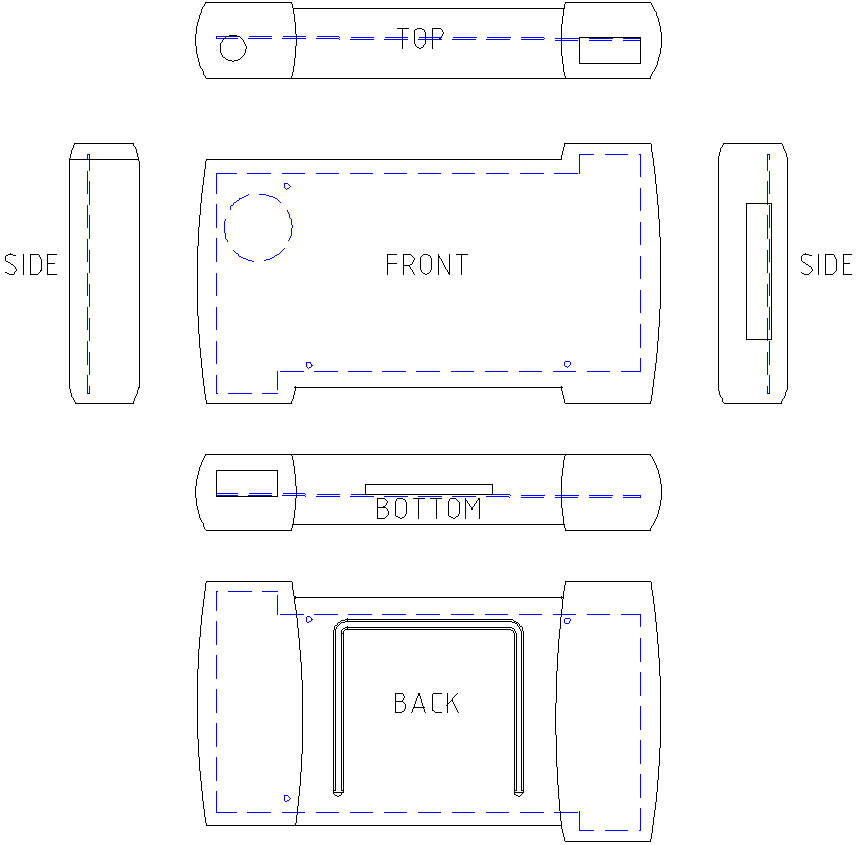
\includegraphics[width=10cm,height=10cm,keepaspectratio]{Figures/design1_sketch.png}
\caption{This is a sketch of the first concept design drawn to the scale of the PCB.}
\label{fig:Design_1}
\end{figure}

The addition of a device stand is intended to support design principle six, in that users can set their device down in a viewable orientation as opposed to potentially having to hold the device for an extended period.
In hindsight, most of this design’s features are quite mundane in that while they account for all major ports and include a device stand to prop it up, in terms of the ergonomics, there are very few stand-out features. 
One thing that can be noted is that the case is compact with a curved profile on either side where the user’s hands are expected to rest which is once again.

%-----------------------------------
%	SUBSECTION 2
%-----------------------------------
\subsection{Second Design}

Following design principle three, the second design was intended to mimic a video game controller in order to conform better to the hand and give users a more intuitive layout in regards to the orientation of the device when in use. 
This concept inhabits this trait arguably to the highest degree in that most users would familiar with a somewhat modern gaming controller conventions and will immediately understand how the device is meant to be held (design principle three).

\begin{figure} [h]
\centering
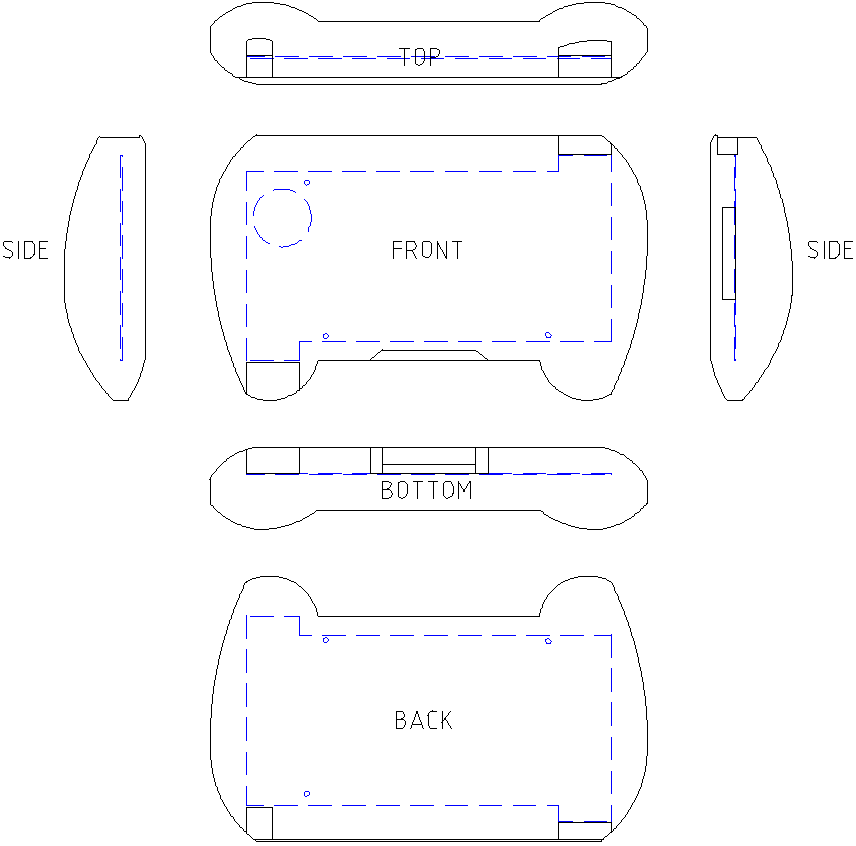
\includegraphics[width=10cm,height=10cm,keepaspectratio]{Figures/design2_sketch.png}
\caption{This is a sketch of the second concept design drawn to the scale of the PCB.}
\label{fig:Design_2}
\end{figure}

%-----------------------------------
%	SUBSECTION 3
%-----------------------------------
\subsection{Final Design}

There were a few factors that made this design the final candidate in which to base the main deliverable of this project.
This approach uses handgrips to subconsciously hint to the user the correct orientation to hold the device, which like design two, supports design principle three.
The use of a stand to prop the device up for an extended period reduces the amount of effort from the user, therefore reducing fatigue much like design one.
For these reasons, this was the design in which the project is based.

\begin{figure} [h]
\centering
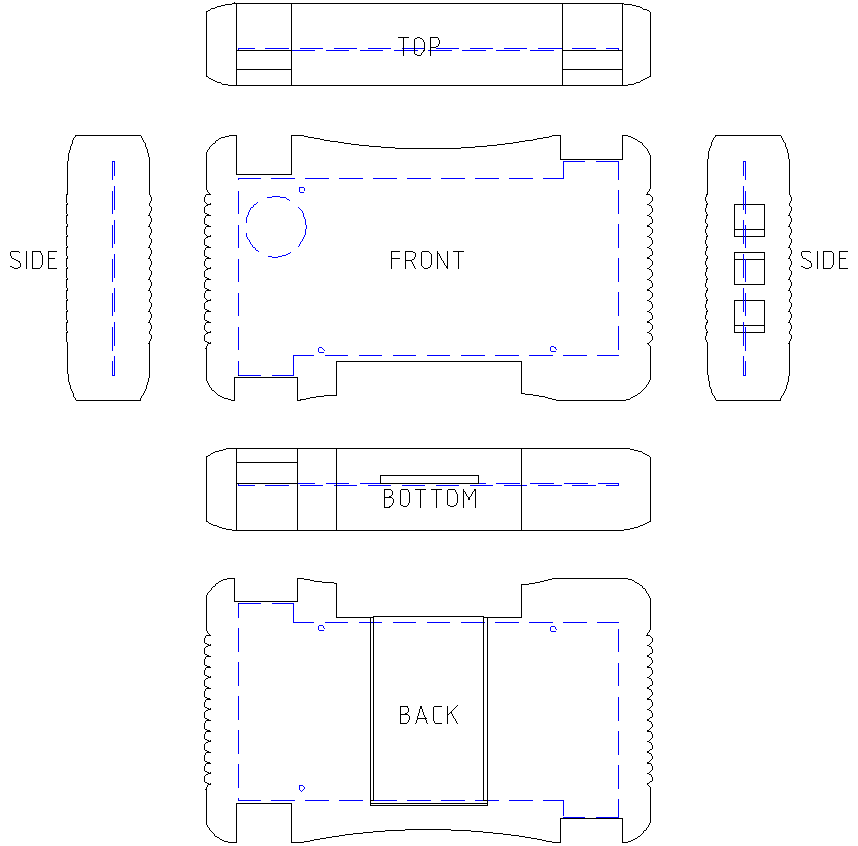
\includegraphics[width=10cm,height=10cm,keepaspectratio]{Figures/design3_sketch.png}
\caption{This is a sketch of the third concept design drawn to the scale of the PCB.}
\label{fig:Design_3}
\end{figure}

%----------------------------------------------------------------------------------------
%	SECTION 3
%----------------------------------------------------------------------------------------
\section{First Revision} \label{First Revision}

This section provides a broad view of the design process with a 'timeline' based approach, making note of the problems and solutions regarding 3D-printed prototypes.
Detailed evaluations of the specific design features of the MEGAphone housing are provided in section 4.

It is very important to reiterate that due to the COVID-19 pandemic, the original plan to organise community focus groups at Novita \cite{novita} in order to receive feedback was not possible, due to health concerns from the organisation, well within reason.
This was instead replaced by feedback from industry experts, ideally to the same effect, however, some sacrifices were made, specifically regarding the ability to compile data on the useability of the device based on feedback from the aforementioned focus group.

Also note that when this chapter refers to the orientation of the device as 'top' or 'bottom', for example, it is assuming that orientation based on the initial concepts presented in section 2.

%-----------------------------------
%	SUBSECTION 1
%-----------------------------------
\subsection{First 3D-print} \label{First Print}

There was a significant issue that was overlooked with the first 3D-printed prototype in that the thought behind orientation of components was flipped.
Electronic components (including connectors) needed more space underneath in order to fit comfortably and the design up until that point had not properly accounted for it.
The orientation of these ports is very important as this dictates how much volume each of the two main case components takes and this was something that was originally not thought of in the correct orientation.
To rectify this issue, changes were made to the depth of the 'top' and 'bottom' case designs so that the bottom component would house most of the internal components, including those cutouts for the ports of the device.

Another aspect that was later modified was the key-chain feature, as this was thought to be quite small.
Considering extra available space, this was expanded both horizontally and vertically as this was later adapted to become a 'housing' for a carry strap, that could potentially double as a key-chain, to strap to the user if desired.
This is discussed in section 4.4.9 in further detail.

\begin{figure} [h]
    \centering
    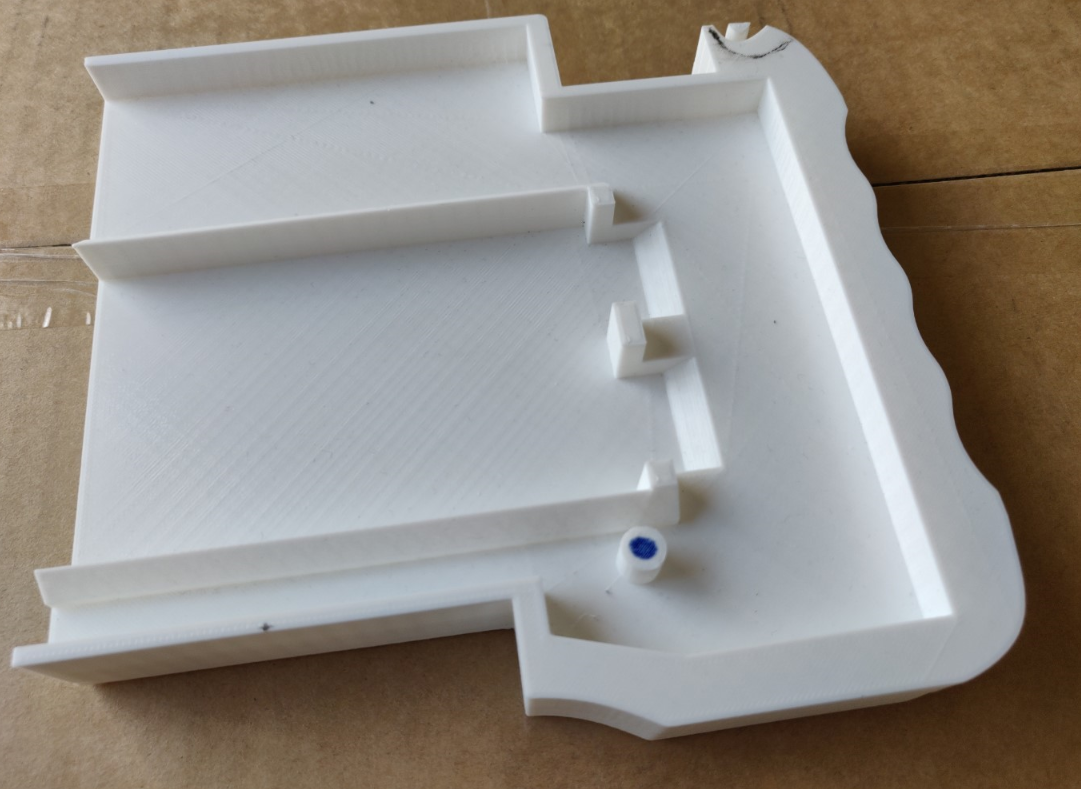
\includegraphics[width=10cm,height=10cm,keepaspectratio]{Figures/firstprint.png}
    \caption{The first print of the 'bottom' case component was sliced due to limited printing space. Markings can be seen where better centring of the PCB was desired and a proposed extension of space around the key-chain feature.}
    \label{fig:First}
\end{figure}

The top half of the MEGAphone housing was not printed at this stage as there was still the concern of where to place the 'EZ access keys' to give users an easier interface than what capable with the Gameboy buttons.
Instead, the plan was to wait until the next stage of the design was complete before going ahead with the next 3D print.

While alignment on the main MEGAphone PCB was correct on the first 3D-print, there was an issue regarding the clearance of the button cutout as well as the positioning of slots to hold the buttons in the correct orientation.
This would be addressed in the next print iteration.

It can also be observed that the 3D print that is the bottom half of the case, featured the battery housing symmetrical with the internals of the device.
This was later changed to make space for the FPGA board, housing the processor for the MEGAphone device, as discussed in section 4.4.6.
% so explain the process of rectifying this issue, map out the impacts and how they are resolved

It is important to note that a 0.15mm print resolution was used, which is not perfect as the project was very precise in some parts, such as the buttons.
Higher resolutions would result in longer print times which makes it impractical.
Silicone injection moulding would present a likely stronger, neater alternative, perhaps when developing a final product.
3D-printing was considered adequate for the task of prototype testing.

%-----------------------------------
%	SUBSECTION 2
%-----------------------------------
\subsection{Second 3D-print}

This section print was where the EZ access keys were implemented, which were considered a vital part of the MEGAphone UD chassis project as they provide one of the more notable appeals of accessibility.
At this stage, another important consideration, the power key, is included and intentionally placed in a button housing that sits at a slightly higher elevation of 0.5mm, to discourage accidental button presses.

\begin{figure} [h]
    \centering
    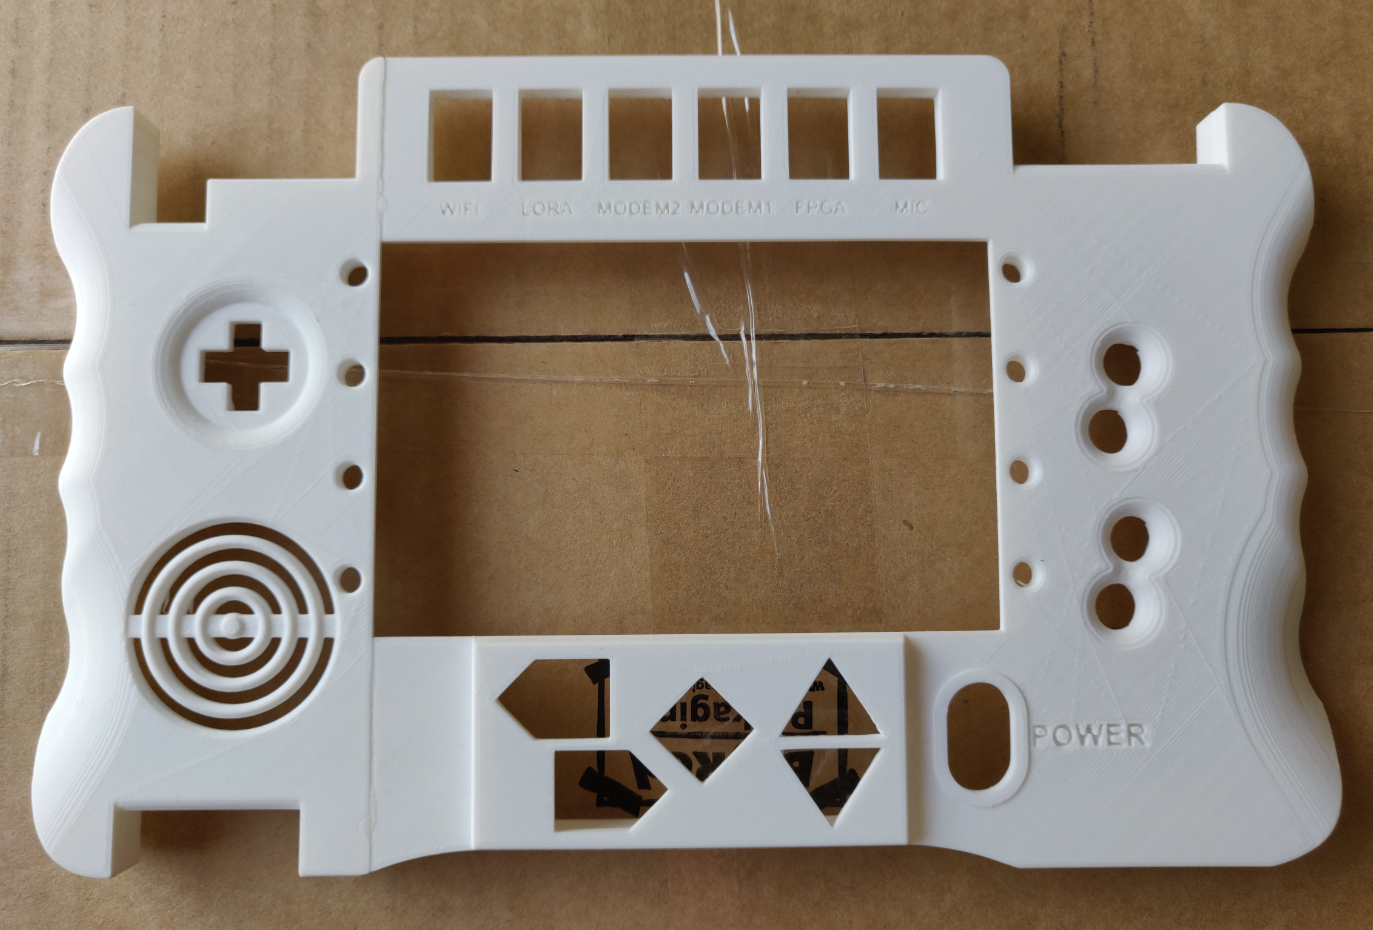
\includegraphics[width=10cm,height=10cm,keepaspectratio]{Figures/secondprint.png}
    \caption{This print was glued together using acrylic glue. Clearance around buttons was not ideal, prompting changes in the next print.}
    \label{fig:Second}
\end{figure}

\begin{figure} [h]
    \centering
    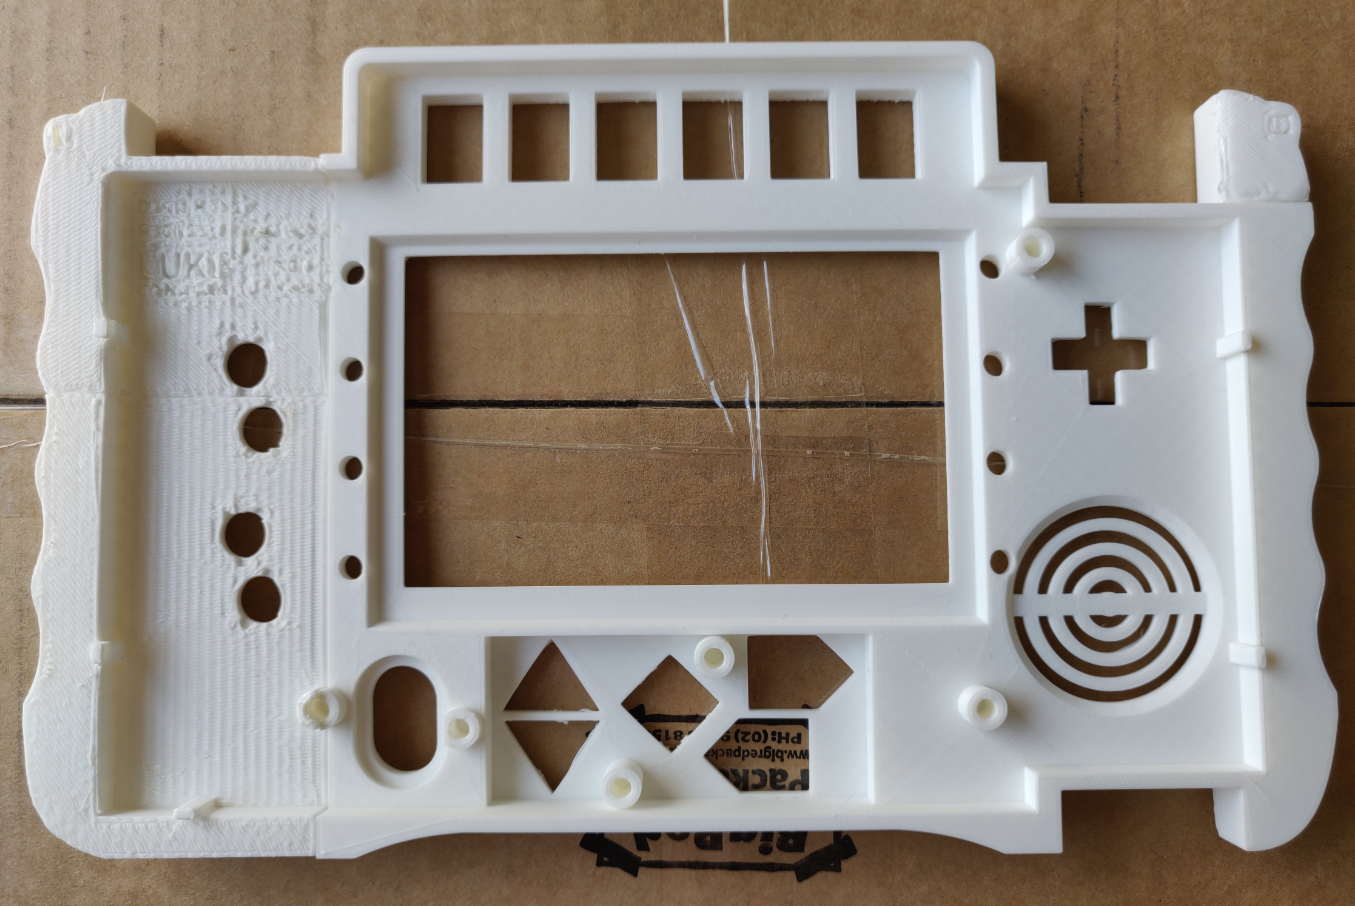
\includegraphics[width=10cm,height=10cm,keepaspectratio]{Figures/secondtothirdprint.png}
    \caption{This print was similar in spec to the previous however, the majority was printed 'upside down' to better highlight the interior. A clearance of 4.25mm for these mounting points allows for M3 threaded inserts.}
    \label{fig:Secondtothird}
\end{figure}

These button housings were not ideal as they provided very little clearance for the buttons themselves.
This was solved in the final print by increasing those openings by 0.3mm in order to allow slightly more space so that actuation was smooth but also ensured that the buttons remain in place.

These prototypes were printed using the Ultimaker 2+, which set size constraints, meaning that the print had to be sliced into multiple parts.

%-----------------------------------
%	SUBSECTION 3
%-----------------------------------
\subsection{Final 3D-print} \label{FinalPrint}

This is the final 3D-printed deliverable of the project and is naturally the most refined revision of the project. 
There are still aspects of the MEGAphone housing that are not perfect as is the case in any iterative design project and the result of this print encouraged changes that are talked about in detail in chapter 5.

\begin{figure} [h]
    \centering
    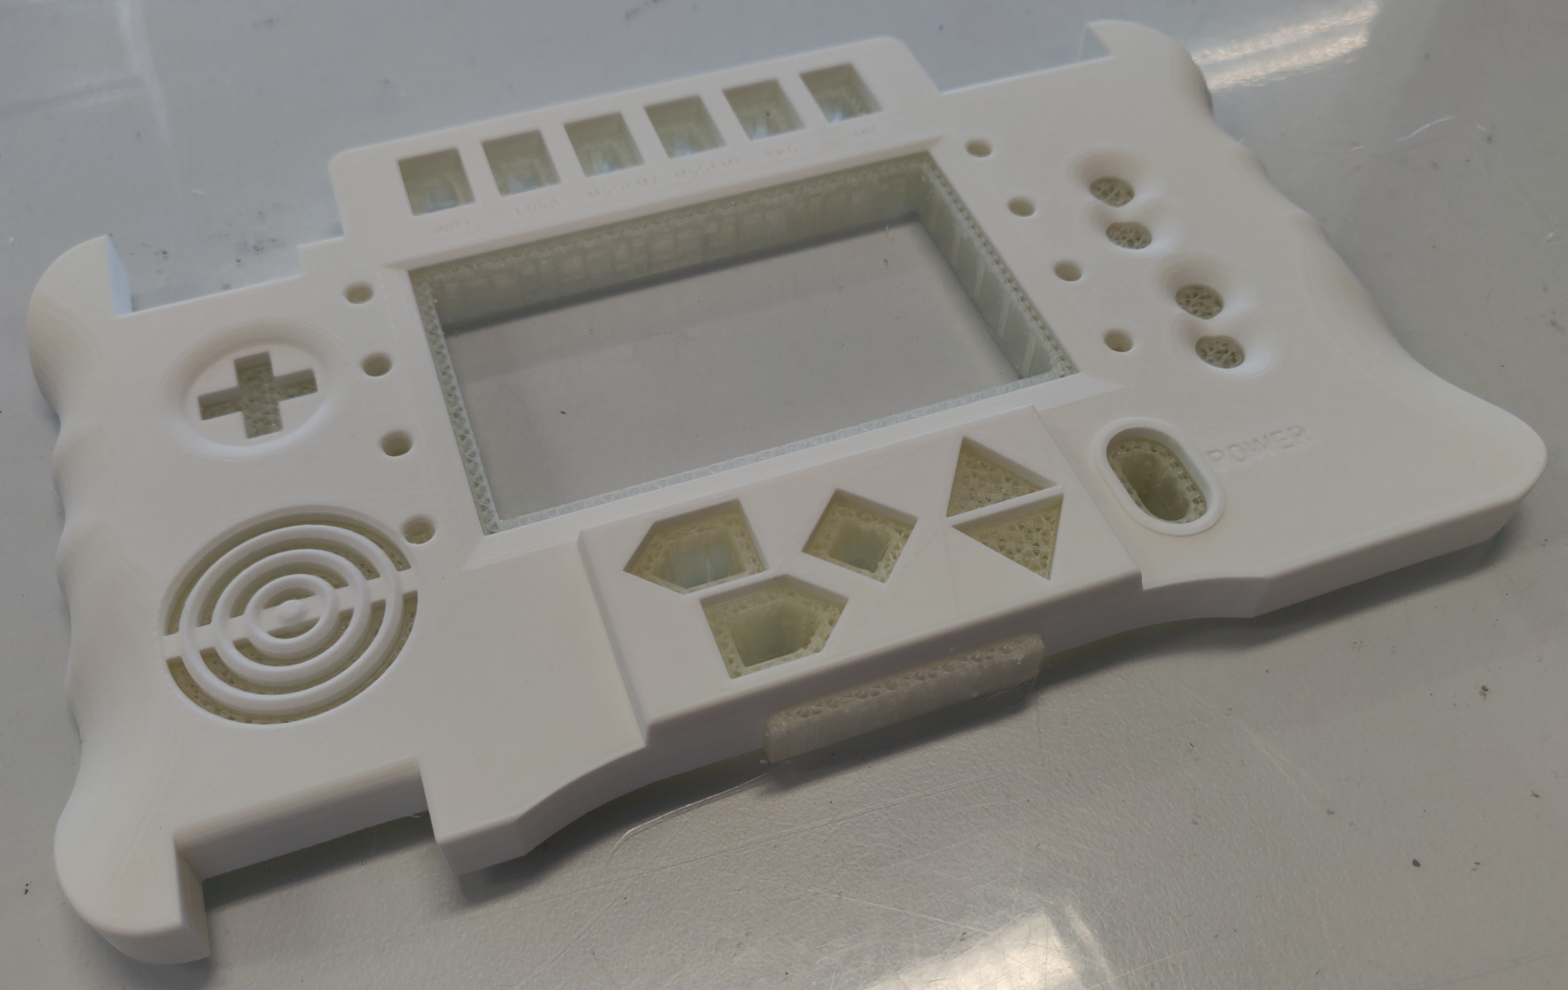
\includegraphics[width=10cm,height=10cm,keepaspectratio]{Figures/topwatersupport.png}
    \caption{This is the final 'top' component print, where water dissolvable supports are visible from the Ultimaker S5 printer.}
    \label{fig:thirdtop}
\end{figure}

Other considerations made to rectify issues in the design, included giving more clearance to the device stand (discussed more in section 4.4.7) so that it could also actuate smoothly and more clearance to the mating fit on the device strap feature.
The latter should have worked and was more likely made an issue due to the inaccuracy of the 3D-printer, nonetheless, considerations were made to increase the opening for this fit.
Giving the battery an opening to easily pick up and set down the device was realised after this print in addition to a housing for a velcro strap to hold the battery in place as sticking it down is considered a riskier approach.

\begin{figure} [h]
    \centering
    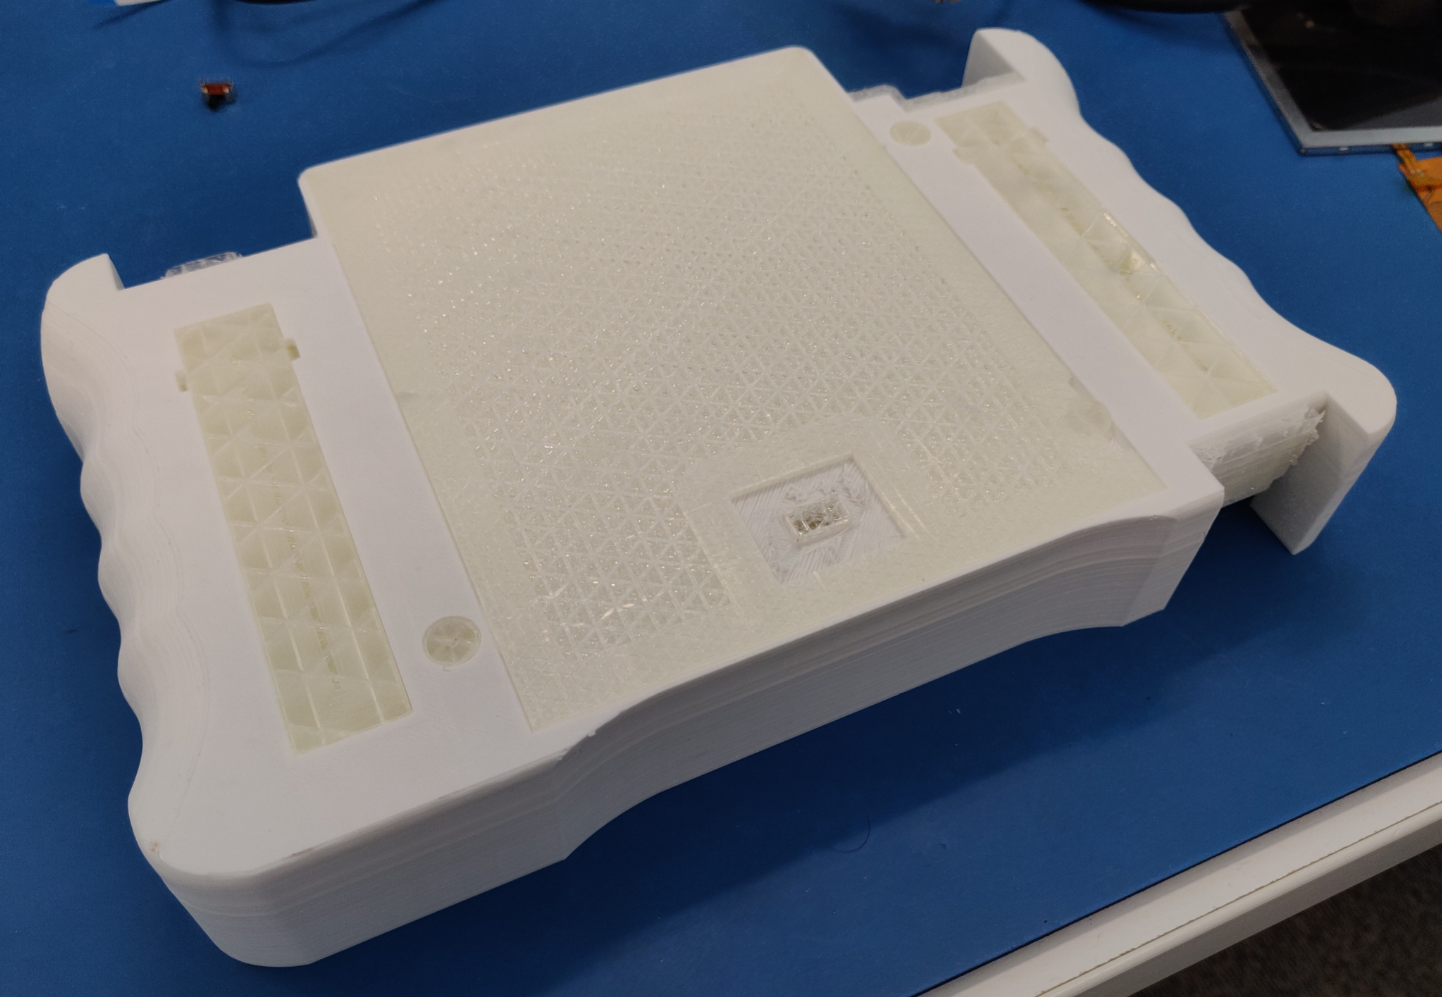
\includegraphics[width=10cm,height=10cm,keepaspectratio]{Figures/bottomwatersupport.png}
    \caption{This is final 'bottom' component where water dissolvable supports can be seen more clearly.}
    \label{fig:thirdbottom}
\end{figure}

This final print used the Ultimaker S5, which allowed a large enough surface area that the entire print was possible without slicing any parts of the case.
Additionally, these prints used water dissolvable supports that dissolve in about one day submerged underwater which made getting to the final product much easier.
The total print time for the final top and bottom case housing was 2 days and 13 hours combined, with the complete housing weighting in at 478g.

%----------------------------------------------------------------------------------------
%	SECTION 4
%----------------------------------------------------------------------------------------
\section{Design Features}

The following section covers the development of all specific aspects of the accessible MEGAphone chassis as well as the accompanying hardware such as buttons, PCBs or hinges.
This serves as a deep-dive into the features of the MEGAphone housing that were briefly covered in the previous section.

%-----------------------------------
%	SUBSECTION 1
%-----------------------------------
\subsection{CAD Sketch}

The first stage of design after the initial concepts was the CAD sketching stage which was approached from a top-down perspective (view fig. \ref{fig:Sketch}).
This is the major outline that users will see when looking at the device in the orientation where the display and buttons are visible, in other words, where users would typically interact with the device.

\begin{figure} [h]
    \centering
    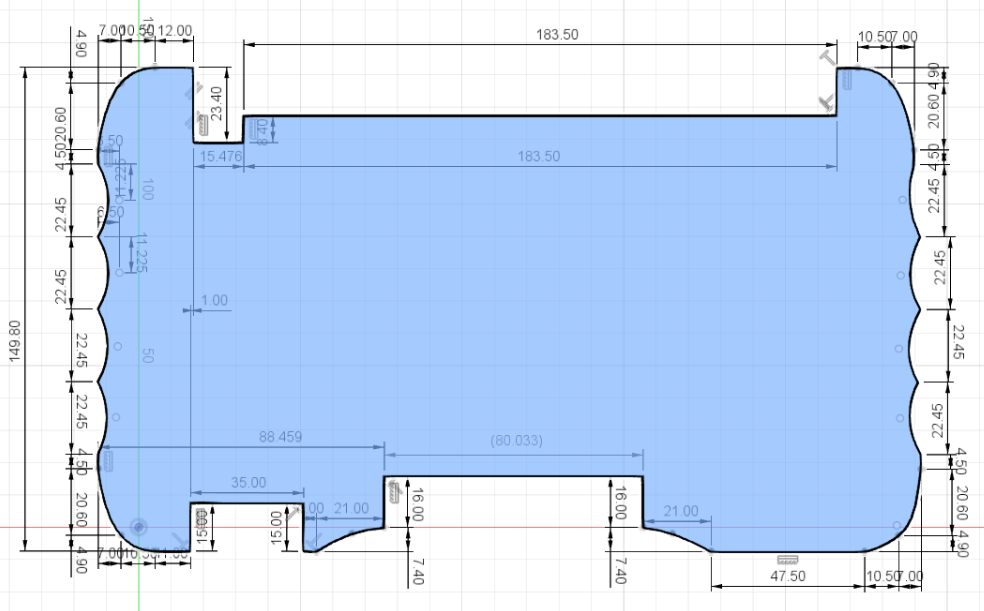
\includegraphics[width=10cm,height=10cm,keepaspectratio]{Figures/blue_sketch.png}
    \caption{The outline sketch of the device is shown.}
    \label{fig:Sketch}
\end{figure}

The outline was extruded outwards in order to create a tangible object in which to mould and add features later on in the process.
Succeeding sketches were simply developed off of this sketch, such as the cutouts for buttons and the display or the hollowed-out interior of the case.
The 'bottom' sketch, for the main accompanying CAD design, was approached in the same fashion where the sketch was extruded outward.
This once again would allow a tangible object in which to add relevant sketches, in the desired orientation.

%-----------------------------------
%	SUBSECTION 2
%-----------------------------------
\subsection{Hand-grips} \label{Handgrip}

The first stage of design after the initial concept sketches was designed to use the 'ridged' rubber grips on both sides of the device (view \ref{fig:old_grips}).
However, this concept was removed in favour of 'ridges' that resemble the size and shape of human adult fingers to more intuitively direct the user to hold the device correctly as this supports the third design principle (view \ref{fig:new_grips}).

\begin{figure} [h]
    \centering
    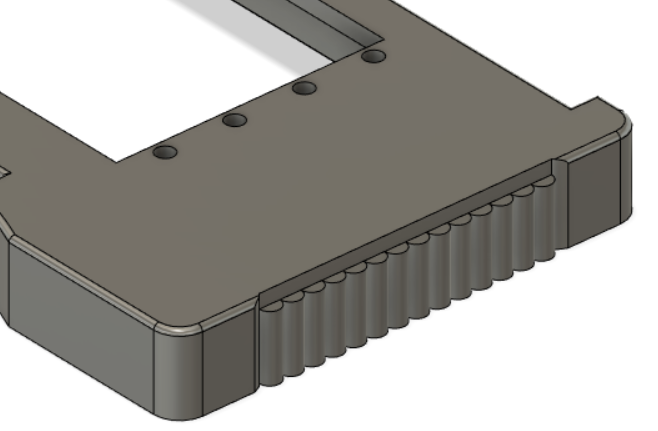
\includegraphics[width=10cm,height=10cm,keepaspectratio]{Figures/handgrip_original.png}
    \caption{This is a model of the original CAD handgrip based on the final design concept.}
    \label{fig:old_grips}
\end{figure}

Another aspect that was considered since the early stages, while less obvious in the final product due to the curved nature, was the introduction of rounded corners as this would minimise hazards to the user.
This was also the case with other edges of the device, in that they were filleted at 1.5mm to remove the sharpness of the device.
Doing adds to the softness from the device and makes it arguably safer for users which is in support of design principle five.
% This was after receiving feedback from my supervisor following an initial design (show design, before and after).

\begin{figure} [h]
    \centering
    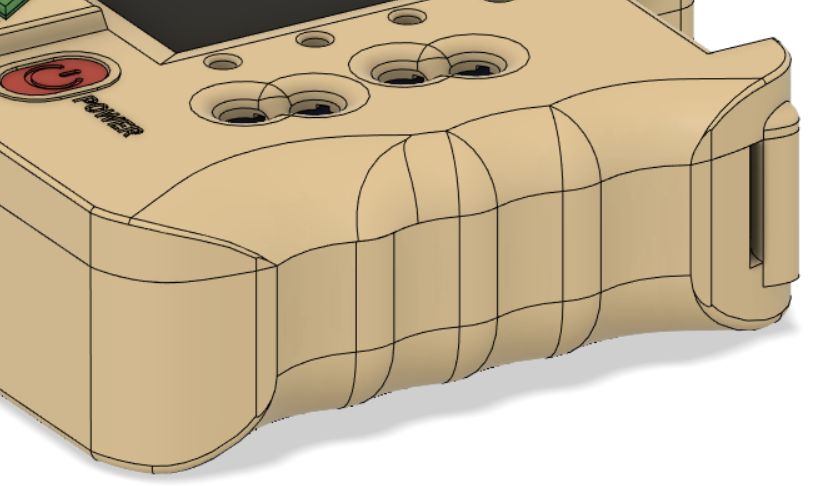
\includegraphics[width=10cm,height=10cm,keepaspectratio]{Figures/handgrip_final.png}
    \caption{The handgrip design was refined by approaching it as something that conforms to the hand rather than just providing a textured surface to hold on to.}
    \label{fig:new_grips}
\end{figure}

A feature that can be noticed in figure \ref{fig:new_grips}, is that the lowest ridge represents a more pronounced 'fillet'.
This design choice was intended as a more defined thumb rest, hinting to the user once again that this is the orientation in which they should place their hands, further supporting design principle three.

%-----------------------------------
%	SUBSECTION 3
%-----------------------------------
\subsection{Rocker Switches} \label{Rocker Switches}

A major issue that was identified from the start with the second revision PCB was that placement and size of switches made it difficult to access.
Larger rocker switches were chosen to be placed on the front surface above the screen as this is in full visibility of the user during use.
These switches relate to the security draw of the MEGAphone device, with insecure modules including, WIFI, Bluetooth, two 4G modems, MEMS mics, LoRa radios and the FPGA serving as the central processing unit of the device.

\begin{figure} [h]
    \centering
    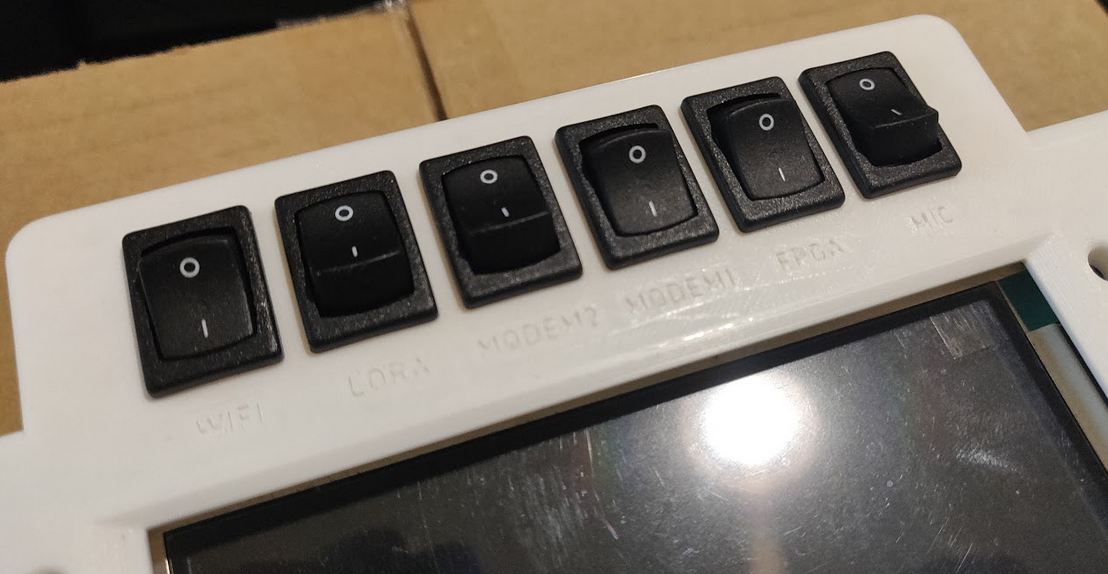
\includegraphics[width=10cm,height=10cm,keepaspectratio]{Figures/hardware_switches.png}
    \caption{The rocker switches, housed in the final product. The labels should be filled in with ink in the final product to enhance readability.}
    \label{fig:Stand}
\end{figure}

The orientation of switches was completely intentional; for easier access for those with limited motor function or even without fingers, having the switches flip vertically would ensure that users are far less likely to flip the wrong switch.
As well as this, the placement of these switches, above the display and away from other buttons on the device ensures that they do not interfere with the operation of the device.
Design principle one and three are satisfied by these rocker switches as they make the security features of this device easily available and the ON/OFF state of wireless modules is made abundantly clear (also supported by LED lights).

An earlier design incorporated the use of standoffs in the design in which to mount the PCB for the switches which was additionally included in the PCB design (view section 4.4). %fix this
This was however later removed in support of design principle three to reduce undesired complexity.
Additionally, it was considered completely unnecessary as when soldered to the switch contacts, the PCB would hold in place, securely and without issue.
On top of this, the rocker switches are placed in from the outside of the device in a press-fit and due to their flat extended base at the 'top', pushing down on the switches beyond a certain point is not possible.

%-----------------------------------
%	SUBSECTION 4
%-----------------------------------
\subsection{Jellybean Switch} \label{Jellybean Switch}

The motivation to include an external digital input switch was to enhance the flexibility of the device (design principle two), as it gives users a new method of interacting with the on-screen keyboard.
The details of the on-screen accessible keyboard are discussed in section 6.

The Jellybean switch sourced for this project interfaces with the device using a 3.5mm Audio Jack connector, a standard feature with accessible switches.
This is very much in the spirit of Microsoft's Xbox Adaptive Controller\cite{adaptive} in that it supports the same standardised connector, allowing a greater degree of adaptability or freedom for the needs of the user.
Another benefit of implementing Jellybean switch accessibility is that it supports the second design principle as it accommodates users who may have great difficulty using the relatively small buttons (which are existing constraints linked to the PCB) or however less likely, the EZ access keys.

\begin{figure} [h]
    \centering
    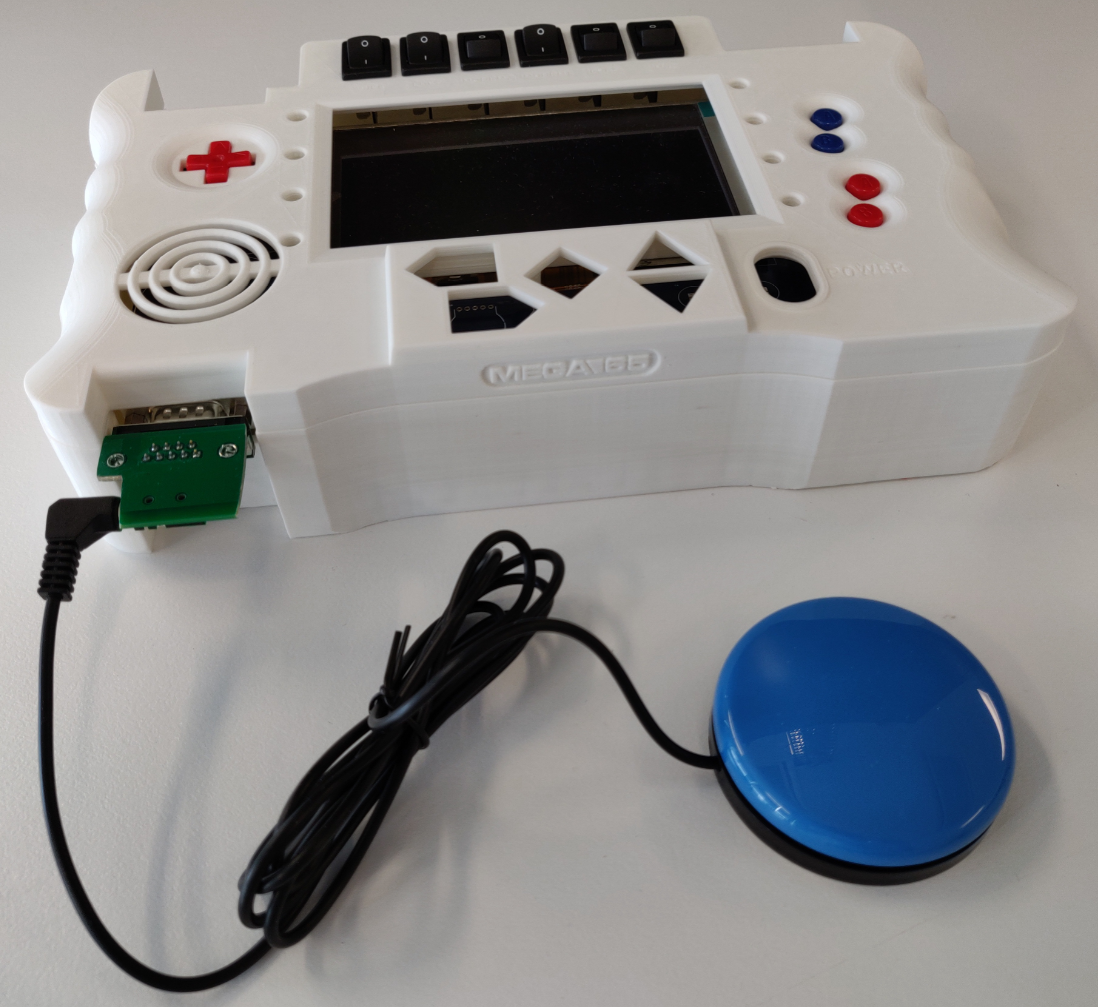
\includegraphics[width=10cm,height=10cm,keepaspectratio]{Figures/jellybean.png}
    \caption{This is a physical example of how the Jellybean switch interfaces with the device during development. Also, a view of the device intact and with Gameboy buttons.}
    \label{fig:Jellybean}
\end{figure}

Given that it is a single digital input device, hardware-implemented accessibility (view section 6) capable of easily communicating with this device was relatively simple to implement. 
The second revision PCB during the commencement of this project did not feature a working 3.5mm Jack connector, therefore, based on this knowledge, the 9-pin DSUB port of the device was hijacked as a single digital input on 'pin 7' for the Jellybean switch. 
% The PCB ‘adapter’ created for this purpose is discussed in section 4.4.
This uses the same pin as the fire button on a retro Commodore64 Joystick controller, hence, integration into the MEGA65 operating system would be straightforward.

%-----------------------------------
%	SUBSECTION 5
%-----------------------------------
\subsection{Recessed Buttons}

% talk about recessing the buttons so that if the device is dropped, minimal/no accidental button presses are registered
% One concept that improves the ‘quality of life’ of this product was the addition of recessed buttons.
There are potential situations where the device might be accidentally dropped which could result in unintended button presses.
The addition of recessed buttons avoids or at least significantly reduces the risk of this situation.
This feature also supports design principle five in that it minimises risks of unintended actions such as accidental button presses, which in this case would be if the user drops the device.
This feature is designed around another existing constraint in that the PCB uses buttons that were repurposed from spare 'Gameboy' parts. %%check this!

%-----------------------------------
%	SUBSECTION 6
%-----------------------------------
\subsection{Battery}

Due to the addition of a new proposed 7.4V 5000mAH Lithium-Ion battery[SOURCE], considerations had to be made regarding placement within the MEGAphone device chassis.
There were two potential approaches to this issue in that the battery could either be placed internally within case along with the electronics, or 'externally' on the 'bottom' of the device with a separate cover that could be screwed on to hide the battery like what might be found on an RC Car controller or TV remote for example.

The approach that was chosen was to have the battery be housed within the case along with the PCBs with the second approach ultimately not being chosen because of three factors.
While the intention of the device is certainly not to be waterproof, there was some desire for the device to protect against light rain, which meant 'sealing' up electronic components at least to some extent.

There is also the concern that the 'bottom' of the device already makes the most of the available space by housing the device stand (view section 3.8) and the solar panel array and therefore the only plausible solution would be to remove the solar panels every time the user requires access to the battery.
As the solar panels would be held in place with an overhang and possibly be stuck down, this would make removing the battery a more painful process.

\begin{figure} [h]
    \centering
    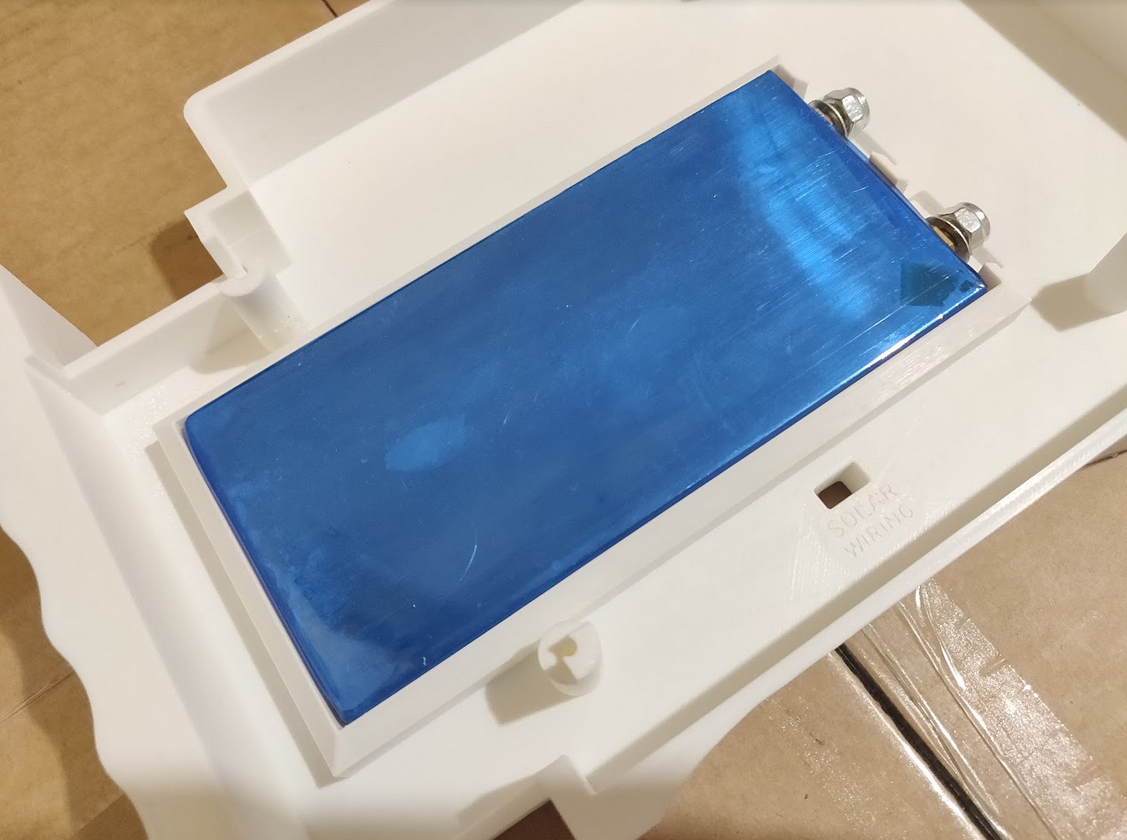
\includegraphics[width=10cm,height=10cm,keepaspectratio]{Figures/battery_housing.png}
    \caption{Here is a photo of one of the batteries seated in the MEGAphone housing.}
    \label{fig:Battery}
\end{figure}

Having the battery be inside within the same compartment as the PCBs, ensures simplicity due to having fewer parts, provides more protection from the elements and as per design principle five and protects users against potential hazards under normal use.
Another motivation for this is that the battery is not expected to be changed regularly and for that reason, having users disassemble the device in this situation is less of an issue as opposed to sacrificing some water 'resistance'.

The battery housing was labelled for clarity and placed asymmetrically to the user's left side due to the location of the bulky FPGA board on the right side of the MEGAphone PCB when looking at it face-up.
This was a change that was addressed in a later stage of development, as the original intention was to place the battery be placed symmetrically on the device as this is best for weight distribution.
In order to not contribute too significantly to the thickness of an already objectively thick device, this was deemed the only reasonable solution to that problem.

This implementation highlights an instance of the relationship that DS and UD can share in that making the device easier to interpret, and manage increases the usability as well as making the repair process easier.

%-----------------------------------
%	SUBSECTION 7
%-----------------------------------
\subsection{Device Stand} \label{Stand}

% thoughts behind the device stand, how they were conceptualised and why it was approached in such and such way; having two stands on either side adds to the stability of the device as opposed to the original idea of having one stand in the middle, which also leaves space for solar panel in the middle
Originally the approach was to have a single 'stand' oriented in the middle of the device where users could extend it out as they need.
However, having two stands on either end of the device has multiple advantages in that doing so increases the stability of the device, as well as giving ample space in the centre to place one or multiple solar panels depending on the available space (discussed in section 3.8).
The mechanism in which to extend and 'lock' the stand in place had the potential to be approached from multiple different angles.

\begin{figure} [h]
    \centering
    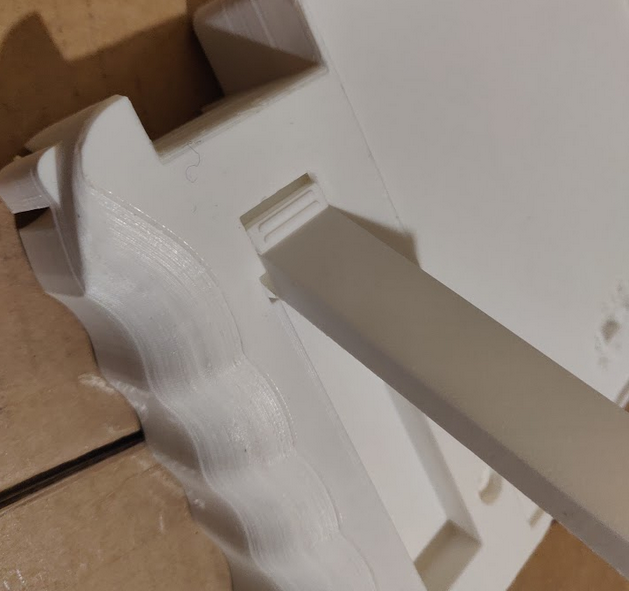
\includegraphics[width=10cm,height=10cm,keepaspectratio]{Figures/stand_housing.png}
    \caption{The MEGAphone housing stand, locked in an extended position.}
    \label{fig:Stand}
\end{figure}

The approach that ended up in the final prototype was to have a sliding mechanism that users could 'slot' in first, followed by a clearance fit in which the stand can rotate around a cylindrical 'mounting' point.  %%show pictures of all this!!
At the opening of the stand where it is expected to assemble with the cylindrical base of the 'mounting' point, a location fit is used, meaning that the user must use mild force in order to get the stand to 'snap' into place.
This ensures that the stand does not fall off the device unintentionally when in normal use.
The aforementioned sliding mechanism slots into two notches which holds the stand in either a horizontal position, flush with the MEGAphone chassis, or an extended position at about 45 degrees so that the device can be propped up under an extended use case.

An alternative that was considered that would have proven to be effective, was to have the cylindrical 'mounting' point in which to revolve the stand, be a part of the stand.
This would almost be a reverse of the actual prototype.
%%add trigonometric function to determine the angle of stand 'foot'

%-----------------------------------
%	SUBSECTION 8
%-----------------------------------
\subsection{Solar Cells} \label{Solar Cells}

% choice of solar panels, discuss potential options and why a specific one was chosen, do a table comparison of available panels and again explain the power output and cost etc.
Giving users more ways to charge their device plays heavily into the DS aspect of this project as this provides a platform in which to harvest energy to power the device without the need for energy infrastructure.
This is something that Gardner-Stephen, in one of his CCC talks, lists as one of the six freedoms to protect against the 'Digital Winter' which Gardner-Stephen refers to as the "situation where the freedoms to create and [innovate] digital systems will become impossible or highly limited" due to reasons listed such as totalitarian governments or failure of critical infrustructure\cite{freedoms}.

The purpose of this is to build toward creating a more self-sovereign device as this not only benefits able-bodied users who expect long-term reliability regardless of external circumstances, but also people with a disability where a more self-sufficient device generally means less effort from the user.
This might be something as simple as being able to leave the device out by a window to charge instead of struggling to insert the charging cable with what little dexterity they might have.
This is an instance of how DS and UD can work hand-in-hand to produce a more convenient electronic platform for everyone.

Seven solar cells from two electronic suppliers, Digikey and Mouser were analysed based on cost, size and energy output for a designated area set out on the MEGAphone case at 125mm by 150mm, collated in table \ref{tab:Solar}.
These panels are all monocrystalline, meaning 'single crystal silicone' as opposed to less efficient, yet more affordable polycrystalline 'multi' options.
The panels will be wired in series in order to generate a compounding power output.
%When a total potential wattage is calculated, it will be divided by the overall cost to determine the best 'power per dollar' option. %%double check maths on this

\begin{table} [h]
    \begin{center}
        \vspace{5mm}
        \caption{Seven solar cells are presented to be analysed for their suitability to a designated space on the MEGAphone case.}
        \label{tab:Solar}
        \begin{tabular}{ |c|c|c|c| }
        \hline
        Product No. & Power Output (mW) & Dimensions (mm) & Cost Per Panel (AU\$) \\
        \hline
        SM301K09L \cite{SM301K09L} & 595 & 58x58x2 & 14.33 \\
        \hline
        SM111K09L \cite{SM111K09L} & 220 & 62x21x2 & 7.17 \\ 
        \hline
        SM101K12L \cite{SM101K12L} & 263 & 45x32x2.1 & 7.08 \\
        \hline
        AM-8801CAR \cite{am8801} & 189 & 58x55x1.1 & 17.65 \\
        \hline
        AM-5412CAR \cite{am5412} & 88 & 50x33x1.8 & 11.61 \\
        \hline
        MP3-25 \cite{mp3} & 90 & 114x24x0.22 & 6.70 \\
        \hline
        MPT4.8-150 \cite{mpt} & 480 & 94x73x0.22 & 20.58 \\
        \hline
        \end{tabular}
    \end{center}
\end{table}

Power (in watts) to area (in millimetres), given the contents of table \ref{tab:Solar} are presented:
\begin{itemize}
    \item Product 'SM301K09L' \cite{SM301K09L} from ANYSOLAR can fit 4 panels into the available (150mm by 125mm) space, netting a total of 2.3W for AU\$28.66
    \item Product 'SM111K09L' \cite{SM111K09L} from ANYSOLAR fits 14 panels into the available space, netting 3W for AU\$100
    \item Product 'SM101K12L' \cite{SM101K12L} from ANYSOLAR fits 9 panels into the available space, netting 2.3W for AU\$63.72
    \item Product 'AM-8801CAR' \cite{am8801} from Panasonic fits 4 panels into the available space, netting 0.8W for AU\$70.60
    \item Product 'AM-5412CAR' \cite{am5412} from Panasonic fits 9 panels into the available space, netting 1.7W for AU\$104.49
    \item Product 'MP3-25' \cite{mp3} from PowerFilm fits 6 panels into the available space, netting 0.5W for AU\$40.20
    \item Product 'MPT4.8-150' \cite{mpt} from PowerFilm fits 2 panels into the available space, netting 1W for AU\$41.16
\end{itemize}

Based on this information, 'SM301K09L' from ANYSOLAR provides the best overall power to cost ratio while 'SM111K09L' from the same manufacturer offers the most power.
The price is, however, exponentially higher for that option, which supports the conclusion that the first choice is far better than all other options considering the specific constraints of the project.
The issue with these options is that none fully satisfy the available area on the MEGAphone chassis as they are not custom made for the device.

Email correspondence with 'Nova Energy' \cite{nova}, the same company that provided batteries for the MEGAphone in the past, quoted a solar cell sample size at 140x125 for US\$10 at 2.4W (AU\$13.60 at time of writing), which is extremely competitive with the other analysed examples.
As supplying directly from the manufacturer cuts out the 'middle man', so to speak, this approach made the most sense, as this would provide the best value for money, at just under half the price of the next best option.
However, generally, these companies act as wholesalers, meaning that they offer these samples with the expectation that their customers will order an extremely large quantity if they are pleased with the quality of their product.
While this sample size would be sufficient for the MEGAphone project, a long term solution to this would be to either buy a much larger quantity or look elsewhere for future samples.

%-----------------------------------
%	SUBSECTION 9
%-----------------------------------
\subsection{Device Strap / Key-chain}

% talk about the process of designing this feature, how the original design changed in favour of larger slot/strap for easier carry
The thought behind the key-chain feature of the device was to be able to clip it to something or fix items to it, and while this feature did see an appearance in an early prototype, it was later adapted into a 'housing' for an arm strap, to allow for easier carrying as this was considered to be more useful.
The reasoning for the original implementation of a key-chain feature was to give users the option to strap the device to their hand in cases where they might have weak grip strength, minimising the risk of dropping the device and supporting the second design principle.

\begin{figure} [h]
    \centering
    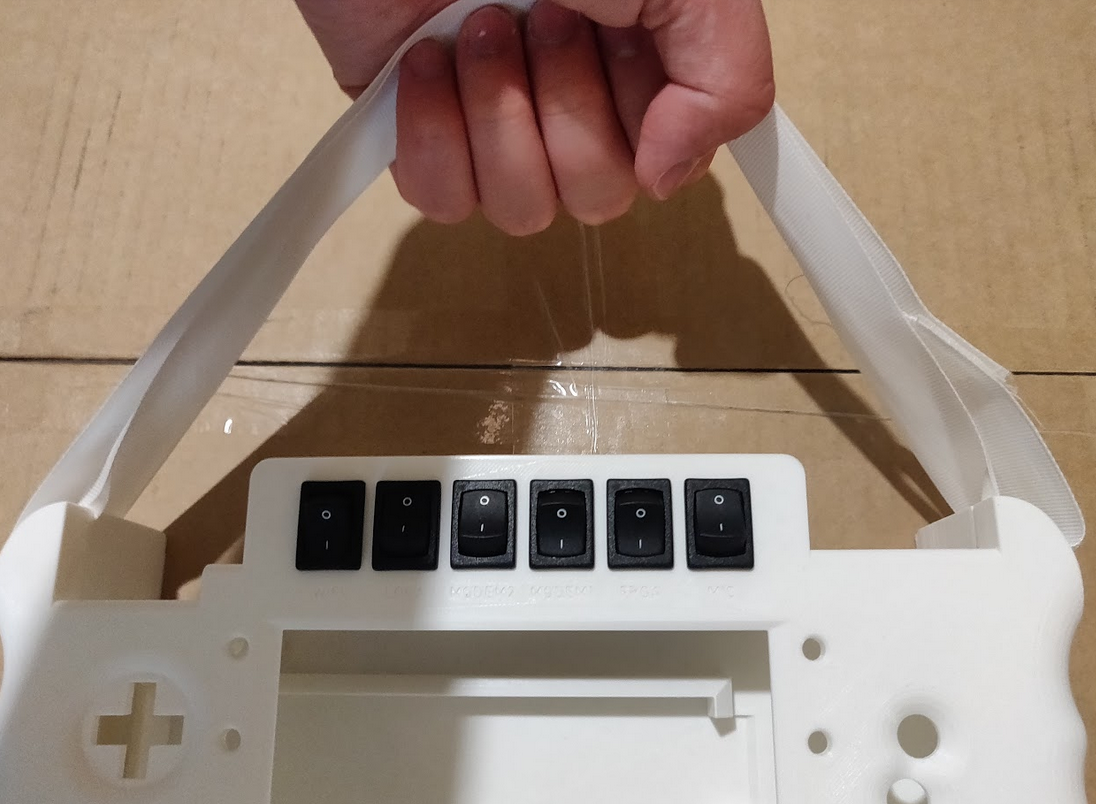
\includegraphics[width=10cm,height=10cm,keepaspectratio]{Figures/carry_strap.png}
    \caption{A proposed way to carry the device might be similar to the image, or a much larger strap to rest on a shoulder.}
    \label{fig:Carry}
\end{figure}

Due to that feature not having many other practical applications in terms of hanging items off of it, the introduction of a much larger opening to integrate a carry strap would better benefit design principle six as it would distribute the weight of the device more evenly when carried.
This would still allow the option for a hand strap, therefore not eliminating that feature.
 
Another consideration was the addition of an extra notch, added to lock into the top part of the case and re-enforce the strength as the entire weight of the device would otherwise be supported by one end of the slot. %%revise, find a better name for 'slot'
The device weighs a little under one kilogram, even at that weight it makes sense to distribute the weight more evenly.

%-----------------------------------
%	SUBSECTION 10
%-----------------------------------
\subsection{Easy Access Keys} \label{EZkeys}

The easy access keys or 'EZ Keys' were inspired by the 'Nav Keys' developed by Storm Interface [source] which feature an array of easily distinguishable keys which were inspired for this adaptation.
These keys benefit from being easily perceptible which envelops design principle four, due to each button not only having a unique colour and shape but also a distinct tactile feel when a button is pressed.

The EZ Keys were first approached as an extension of the device as this would free up a lot of the limited space available.
This would mean making a separate housing and having the device plugged into the 9-pin DSUB port similarly to how the Jellybean switch (see section 3.4, figure X) would interface with the device.
It was ideal for the array of buttons to be integrated into the device as this ensures that the full extent of accessibility is available from the moment the device is picked up.

\begin{figure} [h]
    \centering
    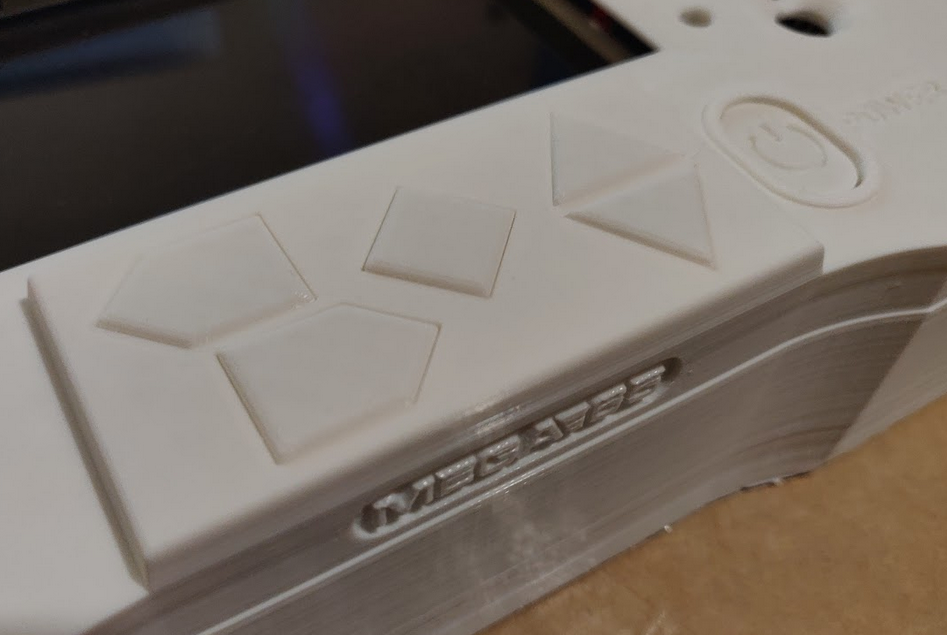
\includegraphics[width=10cm,height=10cm,keepaspectratio]{Figures/easy_keys_housing.png}
    \caption{The MEGAphone 'EZ access' key housing is presented. The final product should be printed in multiple colours to be more perceptible. The MEGA65 logo can also be seen.}
    \label{fig:EZkeys}
\end{figure}

Due to the height requirement of the MEGAphone PCB, there was very little space to attach a slave PCB to allow button functionality, hence one of the reasons why there is an elevation in the button housing.
The second reason for there being an elevation in the EZ key setup is due to the desire to make it more perceptible (design principle four) to users as the position of the power button nearby meant that it would be important to ensure that users do not accidentally press the wrong button (design principle five).
Additionally, there needed to be enough depth so that the PCB could be screwed into place comfortably, elevated slightly above the main MEGAphone PCB as there would be an overlap due to the size and shape of both PCBs.

An issue that came up in the first 3D-print is that the keys did not have enough clearance to actuate without resistance, also in common with the A, B and directional buttons.
This was fixed in an update by extending the width of the button cutouts by approximately 0.3mm as this would also theoretically align with the 0.15mm print resolution. % check this

These EZ Keys serve the DS aspect as they provide a tactile interface that can be used in applications such as disaster relief.
This is evidence that UD and DS share a mutually beneficial relationship.
% FIXED AB AND DIRECTIONAL BUTTON SIZE CLEARANCE, ALSO EZ KEY CLEARANCE
% FIXED ALIGNMENT OF THROUGH HOLE

%-----------------------------------
%	SUBSECTION 11
%-----------------------------------
\subsection{Ventilation} \label{Vents}

% device only uses about 1-2W of power, FPGA using 0.2W
% Not necessary in the final design but add images of version with vents
Thermal management is a concept that came up later in the design process, following feedback at a seminar.
As the MEGAphone device is a low power device by mobile device standards, this was not originally considered vital to the project.

\begin{figure} [h]
    \centering
    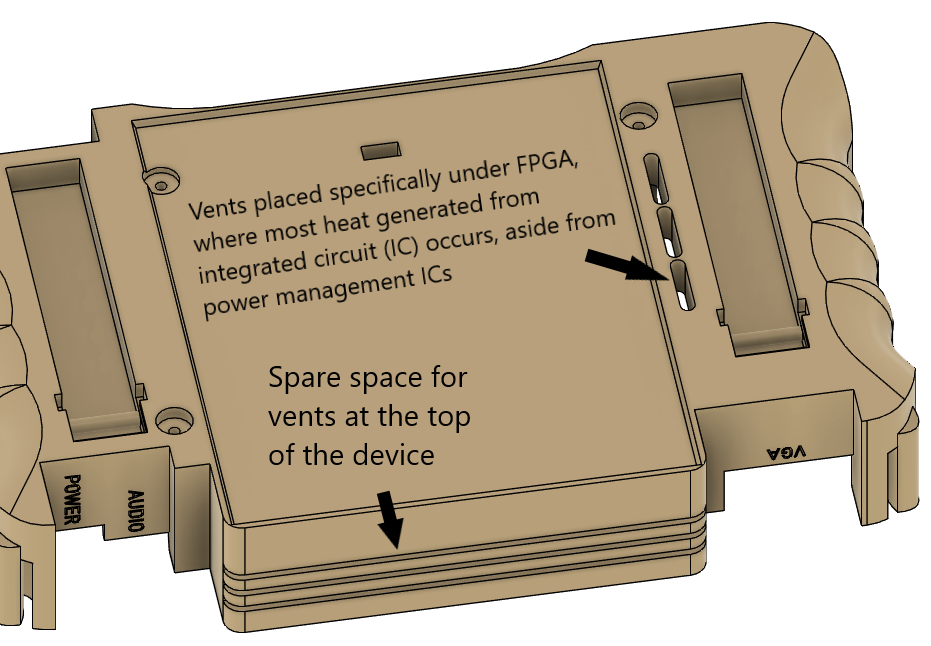
\includegraphics[width=10cm,height=10cm,keepaspectratio]{Figures/ventilation.png}
    \caption{Vents for the MEGAphone device are shown.}
    \label{fig:Vents}
\end{figure}

In its entirety, the device uses approximately 1-2W of power with the heart of the device, the FPGA, using about 0.2W of power.
This yields very little thermal output with the more notable power drawing components being a 110db speaker and full colour 480p display.

However, a consideration for ventilation is shown in figure \ref{fig:Vents}, without a fan setup as this would be considered overkill.
A concern regarding the water-resistance in instances of light rain was brought up, which is why this was not included in the final 3D-print.

%-----------------------------------
%	SUBSECTION 12
%-----------------------------------
\subsection{Potentiometers}

% Slide pot better than thumbwheel pot and explain about physical effort etc.
%% LIKELY GOING IN CHAPTER 5
The potentiometer feature used to control aspects such as speaker volume was a feature that was omitted from the final design due to another more important requirement being the implementation of EZ keys.
This is a feature that can be implemented by other means such as through the EZ keys themselves and therefore a prototype without this would not be a major issue.

The best solution for this would be to employ an array of sliding potentiometers to control any desired functions such as volume control, would be the easiest in terms of the amount of effort that users have to exert and in support of design principle six.
Any potentiometer that is too small or requires a twisting motion would be more difficult for some users, such as elderly users with weaker grip strength.

%-----------------------------------
%	SUBSECTION 13
%-----------------------------------
\subsection{Port Access}

Port access was intentionally designed to have no case material on the top and bottom of the device minimise interference with the plugging in of various peripherals, supporting design principle seven.
These ports are all labelled, explaining in one word the purpose of each port to make it abundantly clear to the user.

An issue that was faced in the original prototype was regarding the orientation of the port cutouts that were placed on the display side of the PCB.
This was rectified by extending out the bottom chassis component with the port cutout on that side so that it would match up with the true orientation of the ports. %expand on this later with images

%-----------------------------------
%	SUBSECTION 14
%-----------------------------------
\subsection{Threaded Inserts} \label{Threaded}

An important aspect of this deliverable is to have a method of securing all parts in place as well as being easily accessible to users who wish to repair or modify certain aspects.
This meant that using a 'pentagon star' screw for example, would not have been a reasonable choice as it would make repair or modification more difficult, due to users not typically having the suitable screwdriver for that job on-hand.
Naturally, this would all be fastened using 'phillips head' screws as these are widely considered the most common screw head type aside from 'flat head' screws.

These constraints were already set out for the MEGAphone PCB in that there are holes in certain parts of the case for this exact purpose.
However, an issue that had to be addressed was the placement of certain components on the PCB and their vicinity to these 'mounting' points.
In particular, one of the MEMS mics, some resistors and transistors were placed closer to this mounting point than what would've been ideal and for this reason, certain parts of the mounting supports were trimmed around these obstacles.

\begin{figure} [h]
    \centering
    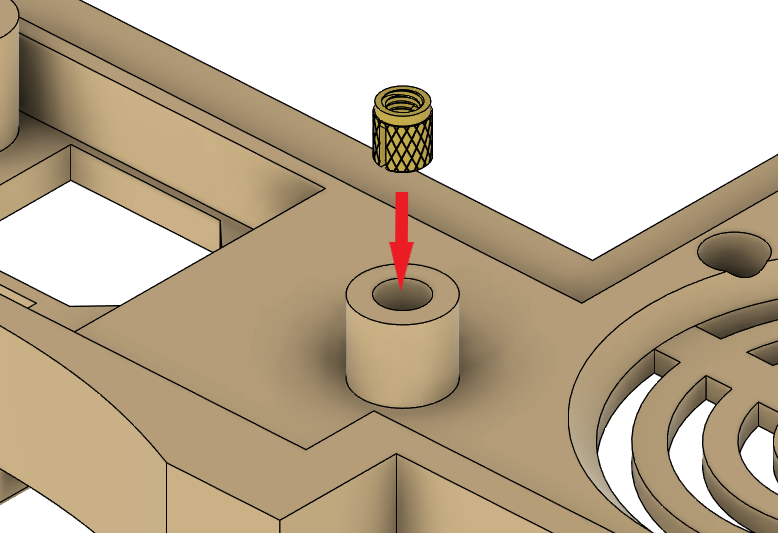
\includegraphics[width=10cm,height=10cm,keepaspectratio]{Figures/threaded_insert.png}
    \caption{Threaded inserts will interface with the MEGAphone as illustrated. The M3 brass insert model in this image is sourced from Grainger \cite{insert}.}
    \label{fig:Threads}
\end{figure}

The alternative that would achieve the same outcome would have been to 3D print solid standoffs and use self-tapping screws in order to securely fasten the device.
This option is however more unreliable as it requires a user-guided input, reasonably soft material and most importantly would require a 100\% 3D infill to be effective, almost doubling the overall print time.

A third option that was disregarded would have been to 3D print the threads, which at a 0.15mm print profile, would have left much room for error considering that this project requires considerably small M3 screws to remain compliant with the constraints of the MEGAphone PCB.
Doing so would also increase the rate of deterioration over brass threaded inserts, due to friction causing wear on the plastic as screws are removed and replaced.

The choice to use threaded inserts for this project was due to its reliability, in that the threads must be consistent due to strict manufacturing standards.
Another reason why they were a solid choice was due to being readily available from any hardware store, making the sourcing of this component very convenient which plays into the DS aspect.

%-----------------------------------
%	SUBSECTION 15
%-----------------------------------
\subsection{MEGAphone PCB}
A new MEGAphone PCB was built up for this project, including sourcing of components and soldering of through-hole and surface-mounted components.
For the most part, very little changes were made from the original two second-revision PCBs, and while one of those two could have certainly been modified to fit these new parameters, external factors meant that those PCBs could not be accessed.

\begin{figure} [h]
    \centering
    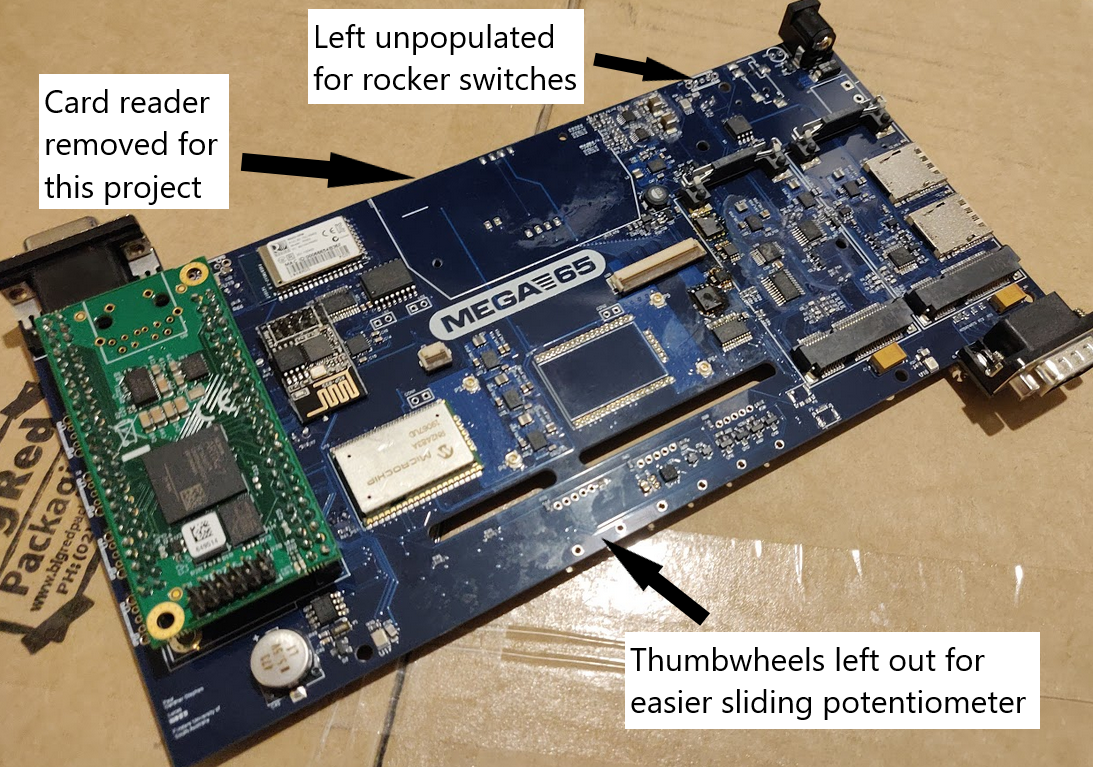
\includegraphics[width=10cm,height=10cm,keepaspectratio]{Figures/megaphone_pcb.png}
    \caption{This is the PCB that was populated for this project.}
    \label{fig:PCB}
\end{figure}

As discussed briefly in section 4.3, the changes made included the addition of rocker switches and therefore the removal of the much smaller slide switches. %%add sources
As well as this, the previously used thumbwheel potentiometers were intentionally left out not only due to the potential to interfere with the EZ access keys PCB due to the very little clearance of 4mm but more so as the desire is to hijack this for testing slide potentiometers in the future.

The implementation of slide potentiometers significantly benefits the usability of the device and while the thumbwheel design works much in the same way, there is currently no realistic way to access it without moving or removing the EZ access key feature which can theoretically be used for the same function by reconfiguring the FPGA.
Not to mention their horizontal placement would mean that they only make sense to be placed on the 'bottom' of the device in the same space as the MEGA65 logo, which from an intuitive use standpoint (design principle three), is not ideal.

%----------------------------------------------------------------------------------------
%	SECTION 5
%----------------------------------------------------------------------------------------

\section{PCB Design} \label{PCBs}
This section discusses the process of designing the supporting PCBs for this project.
These are the PCBs intended to work around the alternative of a costly and time-consuming redesign of the MEGAphone PCB as it was not designed under UD.
As previously discussed, the UD concept is a new introduction to the MEGAphone project.
% explain workaround for previous button layout, using slave boards with tactile switches as well as choice behind contact pads instead of connectors to save space

%-----------------------------------
%	SUBSECTION 1
%-----------------------------------
\subsection{Rocker Switch PCB}

The PCB designed to organise the routing of power to the array of rocker switches originally had the intention of interfacing with the main PCB through a connector of some sort.
With space being a limiting factor, an alternate solution was carried out.
The introduction of 'mounting' pads to serve as a soldering point for the wires would allow them to be comfortably routed to the main PCB.

An issue with the footprint that was observed after sourcing these parts, was that there was not enough clearance for the pins to 'slot' through.
The approach was to file down the pins on the rocker switches individually so that they would fit, which was not an issue in regards to current as the whole device runs on about 1-2W, with a rocker switch[REF] able to handle approximately 2kW of alternating current.
Filing down the PCB through-hole cutout would have made for a far worse alternative as there was potential for the solder to not flow evenly due to damaging the solder mask. %double check this

\begin{figure} [h]
    \centering
    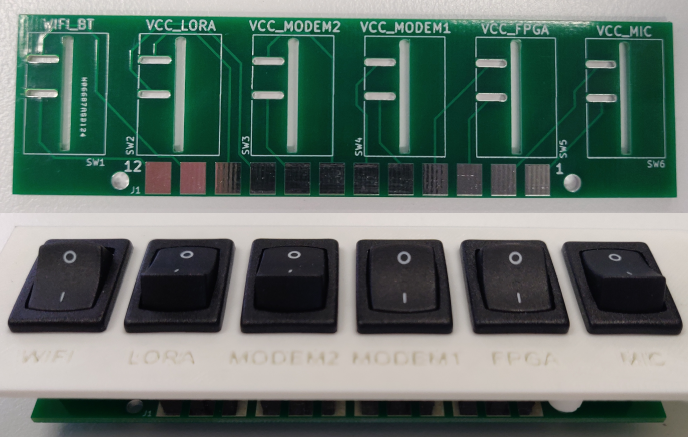
\includegraphics[width=10cm,height=10cm,keepaspectratio]{Figures/rockerswitchpcb.png}
    \caption{This is rocker switch PCB used to interface the rocker switches with the MEGAphone PCB. The PCB above presents the tactile switches while the PCB below shows the pads used to interface with the main PCB.}
    \label{fig:Rocker}
\end{figure}

During the case design process, having mounting points to hold the circuit board in place was implemented.
This was later removed as the switches mount very securely in their cutouts coming from a top-down orientation and so pressing in or flicking these switches would not put any stress on the PCB, unlike the EZ keys in section 4.2.
Doing so allows for adjustment of the PCB, if necessary, before soldering it as well as fewer parts making the repair process easier if users need to replace or modify certain parts.
Clearance between the PCB and the main MEGAphone PCB was additionally very minimal and so the introduction of a bulky connector would make containment of this device far more difficult.

An alternative to this that would have proven effective and arguably neater in a final version would have been to employ the use of a low profile 'ribbon' style connector with separate wires that are thick enough to handle decent current as well as be independently wired to different areas of the MEGAphone PCB.
The reason why this was not chosen is that this deliverable is a proof of concept where the intention is for the MEGAphone PCB to be redesigned so that these rocker switches can be incorporated into the main design, therefore purchasing these connectors for this purpose would be ultimately wasteful.

%-----------------------------------
%	SUBSECTION 2
%-----------------------------------
\subsection{Easy Keys and Power}

The purpose behind the Easy Keys or 'EZ Keys' as otherwise referred to, was to give users a platform in which to interact with the MEGAphone device while being as clear and easy to use as possible.
Multi-coloured, multi-shaped keys are employed make things as unambiguous as possible which include, left and right (forward and backward), up and down, and a 'fire' or enter key.
This, as discussed in section \ref{EZkeys}, is inspired by the Storm Nav-pad \cite{navpad}, where a version has been achieved to a budget, for prototype development. %check typing of nav pad

\begin{figure} [h]
    \centering
    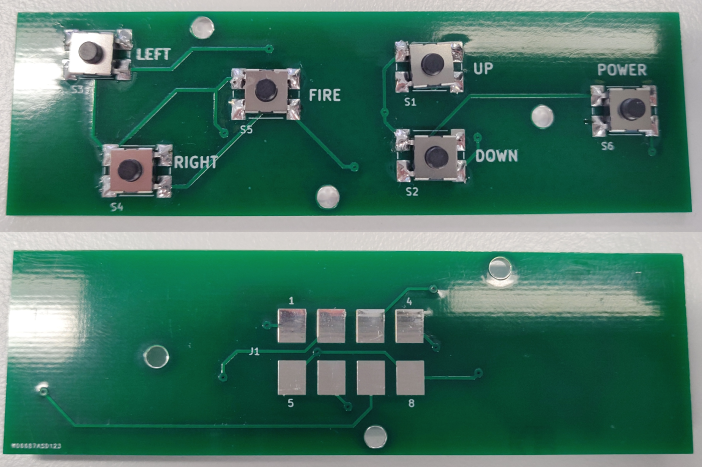
\includegraphics[width=10cm,height=10cm,keepaspectratio]{Figures/easykeypcb.png}
    \caption{The EZ access key PCB used to interface those keys and the power button with the MEGAphone PCB. The layout above shows the PCB with the footprint of the rocker switches, whereas the layout below shows how the switches sit in the MEGAphone case switch housing.}
    \label{fig:EZkeys}
\end{figure}

An important aspect of this device is to provide easy access to the power switch as turning the display on an off on this device is frequent due to not having automatic display dimming features.
This is integrated into the device in the same manner as the EZ Keys, in that they work by momentarily pressing a tactile switch.
These tactile switches are wired directly to the GPIO expander linked to the FPGA on the MEGAphone PCB with the idea being that this new external PCB serves as an extension of the main PCB.

The placement of the pads used to wire the EZ Key PCB was deliberately chosen to be routed to the 'bottom' of the PCB as this would keep the profile of the PCB at a state that is less obtrusive to the rest of the device.
Placing the pads on the 'top' side of the PCB, much like the rocker switches, would have interfered with the space of the display, hence was not considered to be a sensible solution.

%-----------------------------------
%	SUBSECTION 3
%-----------------------------------
\subsection{Audio Jack Adapter}

The audio jack adapter was designed to be a substitute for the original audio jack setup fully integrated on the MEGAphone PCB, which was inoperable at the time.
This PCB hijacks the firing pin of the 9-pin DSUB connector in order to 'imitate' a joystick fire button. 
Coupled with the hardware-implemented features in the FPGA, the MEGA65 OS should treat this input as a regular peripheral such as a Joycon.

An issue that was faced during the development regarded the overall size and shape of the PCB.
This was not thought about correctly at the time of manufacturing as the PCB was too bulky on either side.

The central placement of the audio jack input and the bulky Jellybean switch jack output, meant that interfacing with this adapter was inconvenient.
To fix this, a 'nibbler' tool was used to clip away at the edges to cut the board down to size, followed by a rough 80 grit sanding to smooth the edges somewhat.
Given that fibreglass particles are not good for health when inhaled, this was undertaken responsibly to ensure that these risks were mitigated.

%----------------------------------------------------------------------------------------
%	SECTION 6
%----------------------------------------------------------------------------------------

\section{Software Accessibility} \label{Software Access}
% talk about keyboard accessibility, term ‘android accessibility encapsulation’ discuss this.
% Also mention the program is working in parallel to the software ‘mimicking’ the c64 system so this is not a C program running on MEGA65 but rather on VDHL, a hardware description language
DS covers a broad context, where the overarching concept is about giving users control over their data, which this case, providing the MEGAphone device with accessible software features can be argued as achieving an extent of this project in that it places more control in the hands of the users.
A commonality between DS and UD can be drawn in this context as UD is the concept that drives accessible design which gives more control to the user.
The keyboard 'software' accessibility aspect of this goes hand-in-hand with the Jellybean switch input (view section 3.4) as this is primarily what is used to control this feature, aside from the potential to implement this on an EZ key button by hijacking the same pin.

\begin{figure} [h]
    \centering
    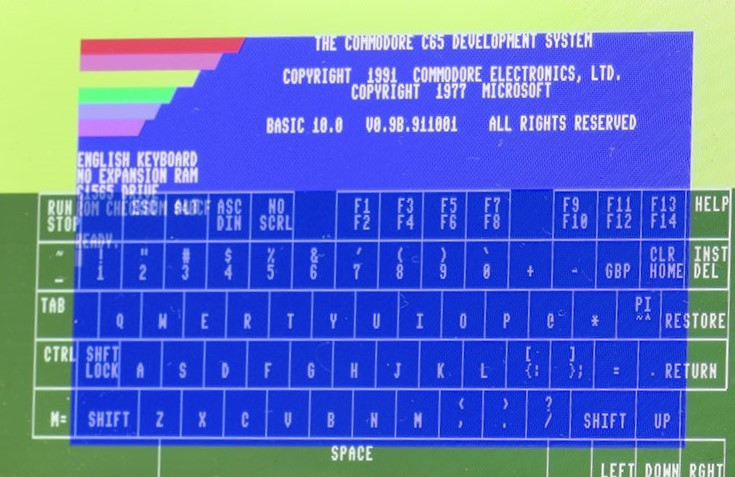
\includegraphics[width=12cm,height=12cm,keepaspectratio]{Figures/keyboard.jpg}
    \caption{This is how the keyboard scrolling feature would theoretically work. Final testing and implementation of the actual software interface was not achieved in the project timeframe.}
    \label{fig:Keyboard}
\end{figure}

As it is coded in VHDL, this is all hardware-implemented in the FPGA which is intended to be completely transparent to the MEGA65 operating system.
This means that the accessible keyboard runs in parallel to the operating system and therefore should not 'see' the Jellybean switch, but instead treat it as if it were any peripheral, such as a Commodore64 joycon.
Due to the Jellybean switch being a simple digital input device, this made implementing this feature relatively straightforward.

The approach was to feature a horizontal and vertical scanning feature for the MEGA65 keyboard which would respond to button presses from the Jellybean input.
Vertical scanning should loop indefinitely at a reasonable pace of one second per key until a button press is registered, in which case, vertical scanning should stop to allow horizontal scanning to begin.
When a full loop is completed, the interface can assume an accidental press and return to a vertical scan. %%add to this and review code
Additionally, any modifier keys should toggle ON/OFF until an action is completed.

%----------------------------------------------------------------------------------------
%	SECTION 7
%----------------------------------------------------------------------------------------

\section{CAD Models} \label{CAD Models}
This section will provide a visual design progression to better illustrate a broader view of the iterative process of this project.
As COVID-19 affected the way that this project was approached, in that designs were not reviewed by a focus group, these versions are not so much seen as 'iterations' but rather significant points in the design process.
This was the case as correspondence with industry professionals normally occurred on a weekly or fortnightly basis, meaning that changes often ended up being very incremental between these meetings.

3D-printing of prototypes occurred at regular intervals, however, these CAD designs might not necessarily line up perfectly with previously presented prototypes.
Much of the design process involved revision and critique of CAD models as a more economical approach, as not all 'stages' of the design warranted physical testing or examination.

%-----------------------------------
%	SUBSECTION 1
%-----------------------------------
\subsection{First Iteration}

The first iteration was most reminiscent of the final sketch design in section 2.3, in that it shares the same ridged pattern (figure \ref{fig:iteration1_t_f}).
Naturally, this was the intention, until the new approach to make it conform to the hand was chosen.

\begin{figure} [h]
    \centering
    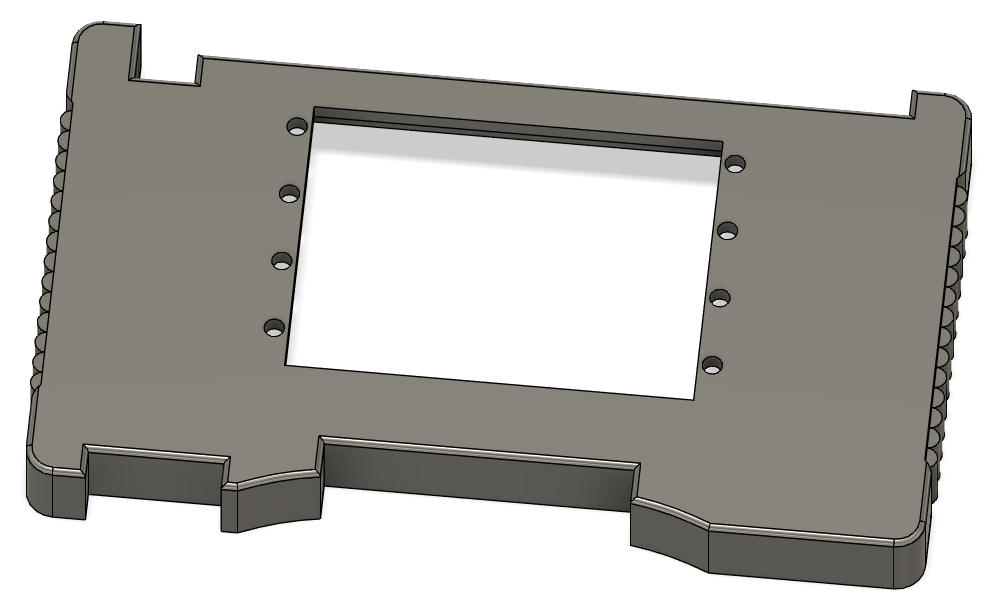
\includegraphics[width=10cm,height=10cm,keepaspectratio]{Figures/iteration1_top_front.png}
    \caption{...}
    \label{fig:iteration1_t_f}
\end{figure}

\begin{figure} [h]
    \centering
    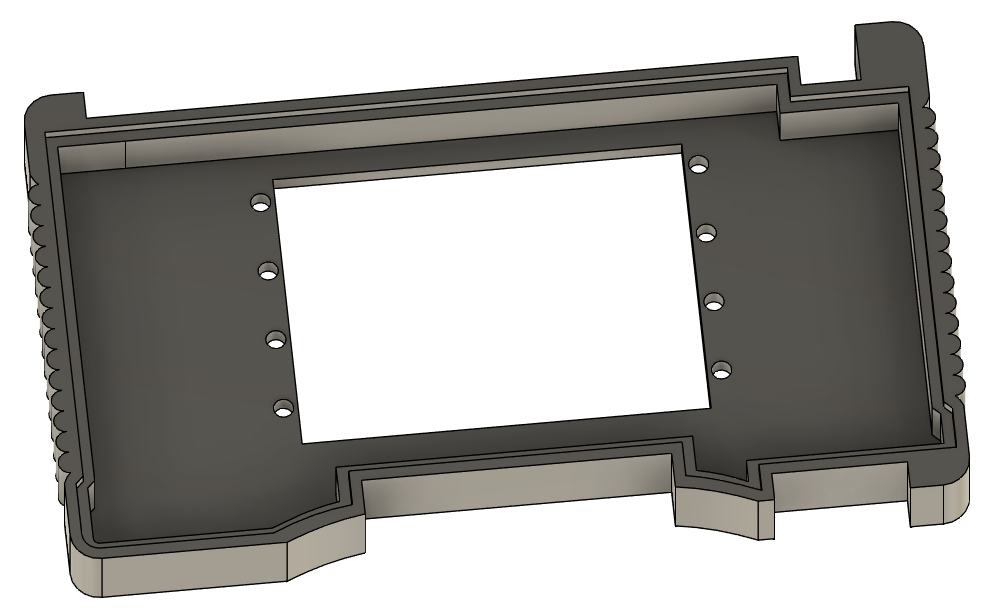
\includegraphics[width=10cm,height=10cm,keepaspectratio]{Figures/iteration1_top_back.png}
    \caption{...}
    \label{fig:iteration1_t_b}
\end{figure}

Underneath the top housing (figure \ref{fig:iteration1_t_b}), a seal can be seen that was intended to mate with the bottom housing.
In the end, this was removed as it was considered unnecessary.
If the intention in the future is to make the device more water-resistant, this option could be employed with rubber seals, however, future iterations of this aspect was considered adequate as it serves its function of holding the two components in place.
Additionally, manufacturing a seal for this would not be considered in the scope of the project and the housing would nonetheless be screwed in to remain secure.

%-----------------------------------
%	SUBSECTION 2
%-----------------------------------
\subsection{Second Iteration}

One notable issue that was addressed in this iteration was the positioning of the openings for the device ports, as seen in figure \ref{fig:iteration2_t_f} and figure \ref{fig:iteration2_t_b}.
As can be seen in the aforementioned figures, the new shape of the device now conforms to the hand,
Other features include the addition of the rocker switch housing at the top of the device, which was later refined to make more space to better accommodate the rocker switch PCB.

\begin{figure} [h]
    \centering
    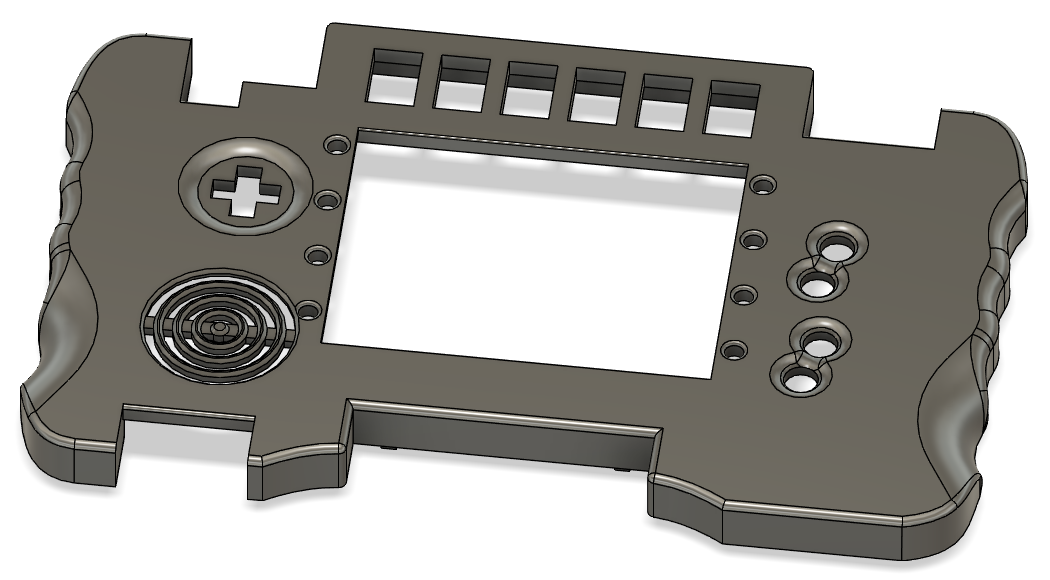
\includegraphics[width=10cm,height=10cm,keepaspectratio]{Figures/iteration2_top_front.png}
    \caption{...}
    \label{fig:iteration2_t_f}
\end{figure}

Other rudimentary, yet key features that were implemented at this stage were the housings for the speaker, DPAD and A, B buttons.
The original key-chain feature can be seen in the top left of figure \ref{fig:iteration2_t_b}, before being swapped for the larger device strap.
At this stage, the bottom housing for the MEGAphone was in development following the re-design.

\begin{figure} [h]
    \centering
    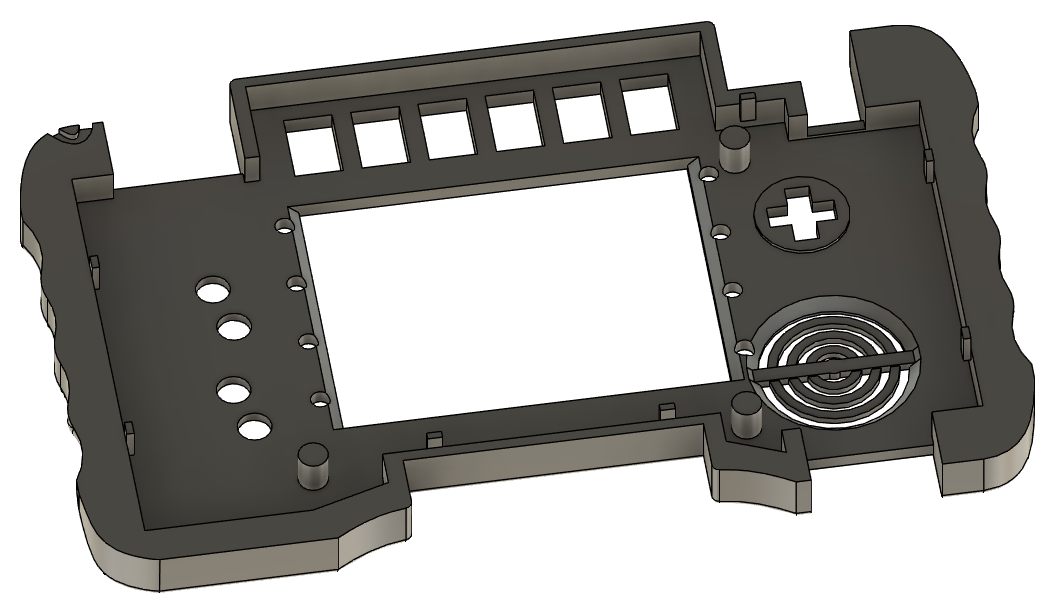
\includegraphics[width=10cm,height=10cm,keepaspectratio]{Figures/iteration2_top_back.png}
    \caption{...}
    \label{fig:iteration2_t_b}
\end{figure}

%-----------------------------------
%	SUBSECTION 3
%-----------------------------------
\subsection{Third Iteration}

The two most prominent aspects of this iteration were the addition of the EZ access keys and the power and LED switches.
Originally the intention was to keep the LED ON/OFF switches, however, it was decided that space could be more valuably used by reclaiming that space for a power only button, as this better supports the useability of the device.

\begin{figure} [h]
    \centering
    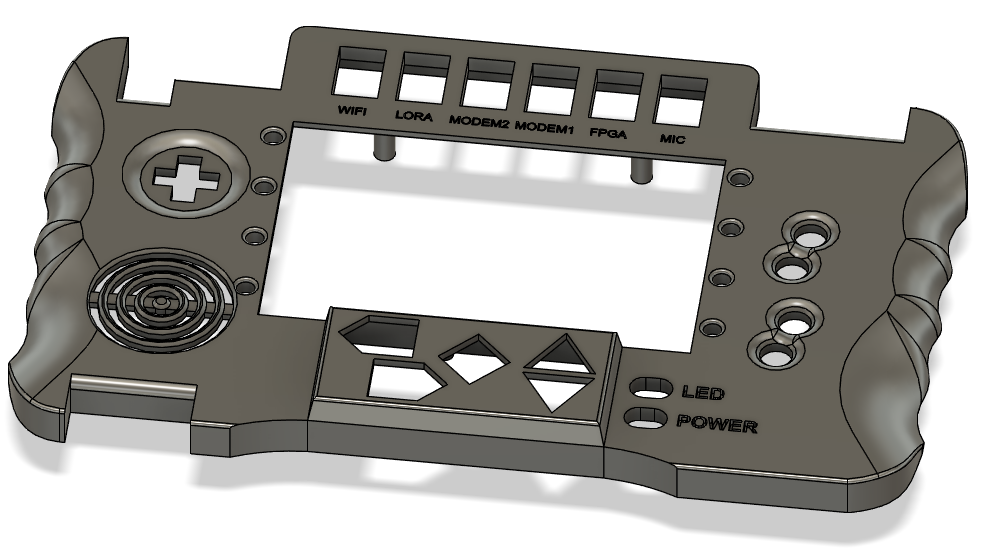
\includegraphics[width=10cm,height=10cm,keepaspectratio]{Figures/iteration3_top_front.png}
    \caption{...}
    \label{fig:iteration3_t_f}
\end{figure}

This supports design principle three as is puts more emphasis on the power button, a feature that is considerably more important than the LED button, as it provides users with the only way of turning the display of due to no auto-dimming capability.
One last note is that this is the only iteration where mounting points up top for the rocker switches as it was deemed not necessary (view section 5.1).

\begin{figure} [h]
    \centering
    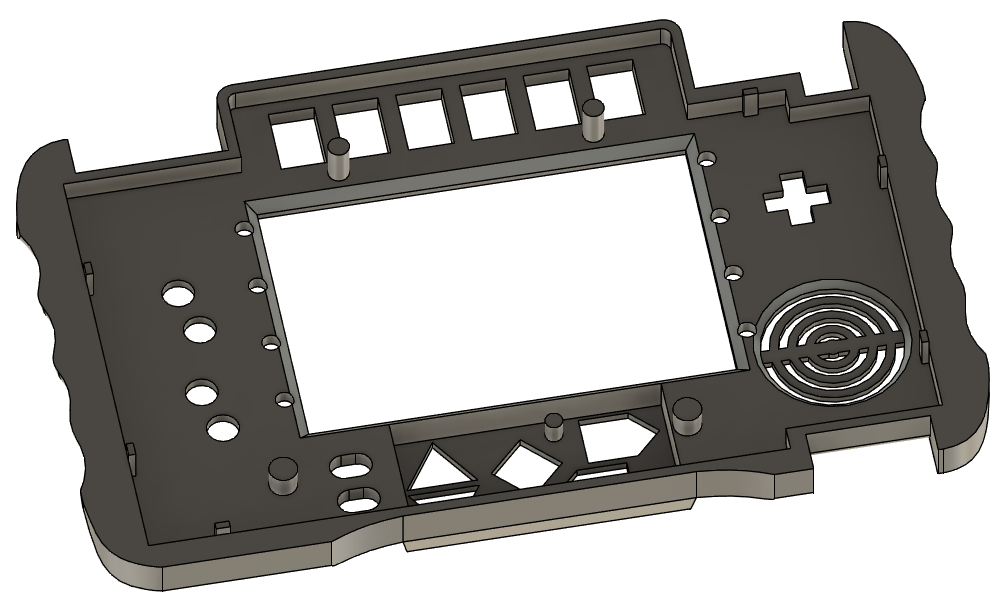
\includegraphics[width=10cm,height=10cm,keepaspectratio]{Figures/iteration3_top_back.png}
    \caption{...}
    \label{fig:iteration3_t_b}
\end{figure}

%-----------------------------------
%	SUBSECTION 4
%-----------------------------------
\subsection{Forth Iteration}

In this final iteration in line with the final 3D-print, it can be observed that a beige colour was chosen as this was intended to relate to the Commodore64 style, although the colour here can be considered much more 'bright' (view figure \ref{fig:iteration4_t_f} and figure \ref{fig:iteration4_t_b}).
Other features include, updated mounts for M3 threaded inserts, guides for the orientation of the A, B buttons, a larger housing for the power button and bezels for the central 480p display.

\begin{figure} [h]
    \centering
    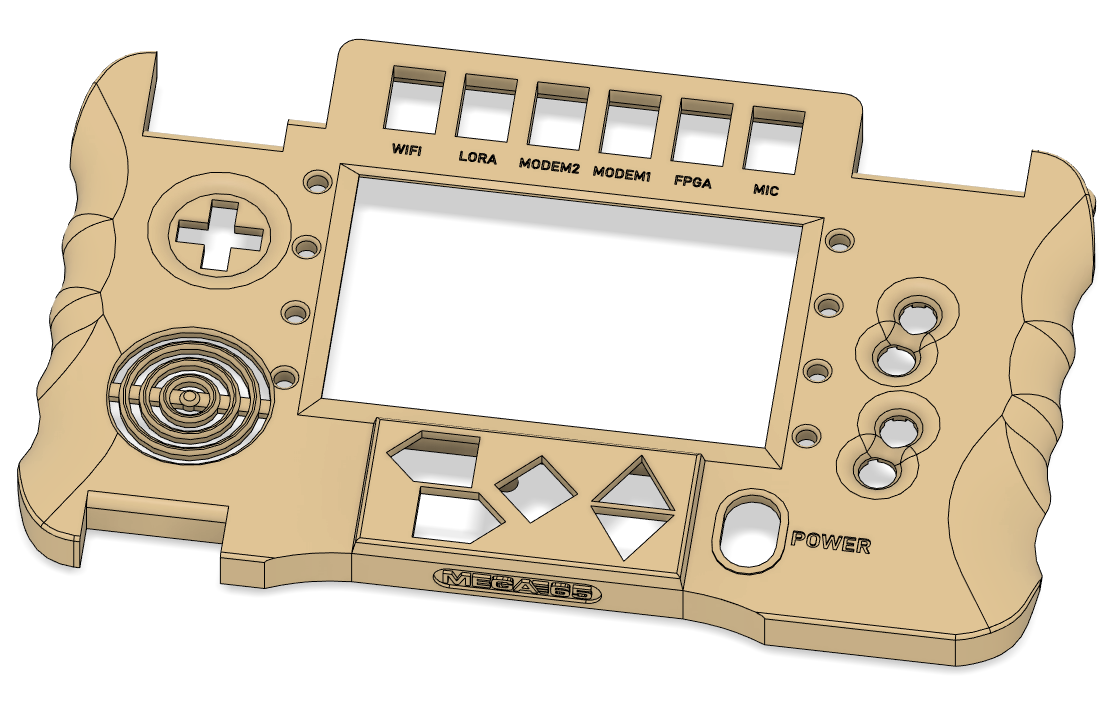
\includegraphics[width=10cm,height=10cm,keepaspectratio]{Figures/iteration4_top_front.png}
    \caption{...}
    \label{fig:iteration4_t_f}
\end{figure}

\begin{figure} [h]
    \centering
    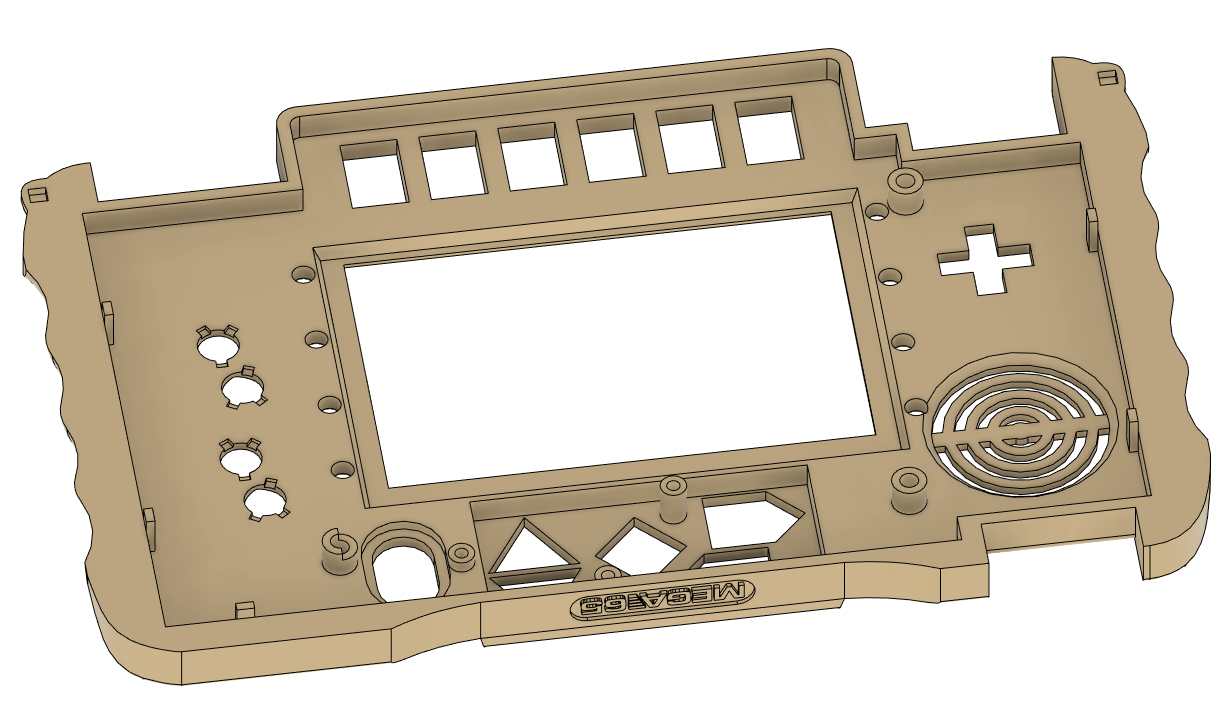
\includegraphics[width=10cm,height=10cm,keepaspectratio]{Figures/iteration4_top_back.png}
    \caption{...}
    \label{fig:iteration4_t_b}
\end{figure}

%-----------------------------------
%	SUBSECTION 4
%-----------------------------------
\subsection{Exploded View}

To better illustrate how the internals of the device interface with the MEGAphone housing, figure \ref{fig:Exploded} is presented.

\begin{figure} [h]
    \centering
    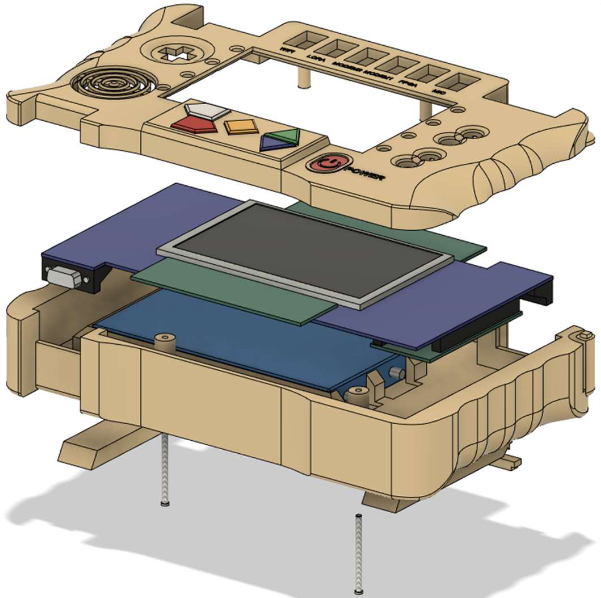
\includegraphics[width=10cm,height=10cm,keepaspectratio]{Figures/exploded_view.png}
    \caption{...}
    \label{fig:Exploded}
\end{figure}

%----------------------------------------------------------------------------------------
%	SECTION 8
%----------------------------------------------------------------------------------------

\section{Summary}  %% TALK ABOUT THE DESIGN IN VARIOUS STAGES, PERHAPS IN A SECTION BEFORE FINISHING TO SHOW THE BIGGER PICTURE
This chapter showcased the development of the universally designed MEGAphone project, highlighting the accessible housing, hardware-implemented accessible keyboard running alongside the MEGA65 OS and the PCBs to adapt a non-UD MEGAphone PCB, avoiding time-consuming and costly redesign.
The next chapter will review the final 3D-printed prototype that this chapter presented and provide CAD designs in support of the critique that the MEGAphone housing receives.
